\chapter{Integration of Pccf with detectors}

\section{Integration of PCCF into a threshold based naive change detector}
\label{sec:pccf_integration_naive}
% From SDM
%\subsection{Integration of an individual change detector with PCCF}
There are two straightforward approaches for using PCCF can be used to potentially improve the accuracy of existing change detectors:
(1)~post-processing -- a detector with fixed settings is used; its output (CDEs) are adjusted based on PCCFs values,
and (2)~pre-processing -- the sensitivity of the detector is dynamically adjusted according to the current PCCFs values.

At the beginning of the change detection process initial probabilities of changes in the foreseeable future are computed using PCCF.
After that PCCF is recalculated every time the last confirmed $c_i$ is known.

In case of post-processing, a change detector with fixed settings, learned offline, is applied.
When the detector alarms a change at time $t$, we check whether the probability of change given by PCCF is greater than a user defined threshold $\mathcal{P}(t) > p_h$.
If it is, we count CDE as a change and output $\Event{t}{+}$, otherwise we output $\Event{t}{-}$.

In case of pre-processing, detector's settings are adjusted dynamically according to PCCF. The detector is made more sensitive when a change is expected with a higher probability $\mathcal{P}(t) > p_h$, and less sensitive when the change is expected with a lower probability.
This strategy should be applied with caution in order not to make the detector too sensitive, which would result in an increase the FP rate.
In this study we consider only scenario when the highest value of the dynamically adjusted sensitivity of the detector is equal to the optimal threshold value learned during the training phase.
When the estimated probability of the change given by PCCF is low, the sensitivity threshold is lowered.
This scenario is illustrated in Figure~\ref{fig:naivedetector} where detector's sensitivity is a function of PCCF.

\subsection{Experiments}
\label{subsec:experiments}
To illustrate the utility of the PCCF we performed three experiments using artificially generated data and two experiments with real data.
\footnote{We have made the code for computing PCCF and running simulations and experiments publicly available at \url{https://github.com/av-maslov/Pccf}.}.
Our goal is to improve the accuracy of online change detection when recurrent changes are expected.
The required information about recurrence is the time intervals between consecutive changes, given as the parameters of the normal distribution $N(\theta = \mu, \sigma)$.
%After the simulation results, we present the fourth part of the experimental study, in which we demonstrate utility of PCCF on two real data sets.

\subsection{PCCF simulation.}
In order to confirm the correctness of the PCCF Eq.~(\ref{eq:pccf_recurren_1}),~(\ref{eq:gaussian_pccf}) expressing the probability to observe a recurrent change at every moment $t$, we performed a simulation by generating sequences of the recurrent changes multiple times and calculating frequencies of occurrence of generated time locations of the changes at each moment of time.
% (see Algorithm~\ref{alg:pccf_sim} in the appendix).
The shape of the obtained curve of frequencies perfectly fits analytically computed PCCF function.

\subsection{Delay of change confirmation.}
In this simulation we illustrate a procedure to estimate maximum delay of change confirmation $D$ during which the recurrence information in a form of parameters $\theta = (\mu, \sigma)$ is still useful and demonstrate the use of PCCF in post-processing settings.

From Figures~\ref{fig:pccf_example} and~\ref{fig:conffunction} depicting behavior of the PCCF it can be seen that the probability of a change oscillates with decreasing amplitude and converges to the limit $L$.
Assuming the probability of making a FP at any moment is constant and is equal to $\lambda$, there are three scenarios to consider:
\begin{enumerate}
\setlength\itemsep{0pt}
\item The error rate $\lambda$ is higher than $\mathcal{P}(t)$ for all $t$.
In this case the detection accuracy cannot be improved with recurrence information $\theta$;
\item $\lambda$ is higher than the limit $L$ but it is lower than the local maximums of the PCCF $\mathcal{P}(t)$. This case is depicted in Figure~\ref{fig:conffunction} by the horizontal dashed line with value $0.2$.
\item $\lambda$ is lower than the limit $L$; this case is depicted with the horizontal dashed line with value $0.05$.
\end{enumerate}
We are not interested in the first case because the probability of making errors is so high that the baseline change detector should be optimized better first.
In the second case peaks of $\mathcal{P}(t)$ at moments $t = i \mu$ are higher than $\lambda$ until some moment $D$ (vertical line), after which the probability of the error is always higher than the probability of change.
The third case is equivalent to the first case till the moment when local minimums of $\mathcal{P}(t)$ become always larger than $\lambda$.
These observations suggest that we can determine the maximum tolerable confirmation delay $D$ (Figure~\ref{fig:conffunction}) by computing the PCCF function, estimating the error rate of detector, and finding the last peak of $\mathcal{P}(t)$ which is higher than $\lambda$.
To confirm our hypothesis we run the following experiment.

\emph{Input data description}.
For each delay $D$ in the range from 5 to 300 we generate input signal $500$ times with $50$ recurrent change points with $\mu = 10$ and $\sigma = 0.7$.
%The average distance  between changes and its standard deviation are set to $(\mu = 10, \sigma = 0.7)$.
PCCF $\mathcal{P}(t | \mu, \sigma)$ is calculated and updated after the location of the last change is output with the current delay value $D$.
Change point locations are generated according to Definition~\ref{def:recurrentdefinition}, i.e.\ given  $c_1$, the second change is $c_2 = c_1 + \epsilon_1$, $c_3 = c_2 + \epsilon_3$ and so on,  where $\epsilon_i$ is a sample from the Gaussian distribution. %of the first change $p(c_1|\theta = \mu, \sigma)$.
The error rate defining the expected number of FPs per $\mu$ is set to $\lambda = (0.05, 0.2)$.
Time locations of outliers are sampled from the uniform distribution so that there are $1/\lambda$ outliers per time interval of width $\mu$ where $\lambda$ is the FP rate of the detector.

\emph{Change detector.}
In this and the next simulation for PCCF pre-processing we used artificially generated data streams, in which changes are abrupt step changes in the value of the signal.
We use a simple base-level change detector, the output statistic for which is the first order difference of the signal $(x_2  - x_1, \dots, x_n - x_{n-1})$. Its behaviour is illustrated in Figure~\ref{fig:naivedetector}.
A CDE $\Event{t}{+}$ is alarmed when
\begin{equation}
x_i - x_{i-1} > h
\label{eq:naive_detector}
\end{equation}
%
\emph{Experimental results.}
We measure the accuracy of the detector integrated with PCCF for post-processing settings by calculating its TP and FP rates (not the detector it is used to enhance).
The TP rate is a fraction of changes in the input signal that are identified correctly. The FP rate is a fraction of CDEs that would be FPs if the base-level change detector alone was used without PCCF post-processing.
The results are illustrated in Figure~\ref{fig:combined}.
(The corresponding PCCF can be seen in Figure~\ref{fig:conffunction}.)

The left plot in Figure~\ref{fig:combined} illustrates the case when periodicity is beneficial for any delay, since the error rate $\lambda=0.05$ is low and $L>\lambda$ almost all the time.
By the time when PCCF converges to its limit
all CDEs are considered as changes.
That is why the fraction of correctly predicted changes (bold line) tends to $1$ while the fraction of identified errors tends to $0$ (dotted line).

The right plot illustrates the situation, when recurrence information is beneficial only in some cases, that is when the error rate is lower than the values of PCCF.
The maximum tolerable delay $D$ is illustrated by the vertical line. Please observe that this line is located close to the moments when TP rate goes down \emph{and} FP rate goes up meaning that improvement of the base detector is not possible any more. This confirms our hypothesis that the maximum change confirmation delay $D$ can be estimated by finding the closest local maximum of the PCCF which is higher than $\lambda$.
\begin{figure}[htb!]
\centering
\includestandalone[width=0.45\textwidth]{articles/pics/sdm_paper/artificialsig}
\caption{
	The base-level detector.
The lower is the threshold the higher is the probability of error.
Outliers between changes $c_1$, $c_2$ and $c_3$ are detected as changes when using constant value threshold $h_1$.
The optimal dynamic threshold is depicted by the dashed line. }
\label{fig:naivedetector}
\end{figure}
%
\begin{figure}[htb!]
\centering
\includegraphics[ width=0.24\textwidth]{articles/pics/sdm_paper/performance2sdm.pdf}
\includegraphics[ width=0.24\textwidth]{articles/pics/sdm_paper/performance1sdm.pdf}
\caption{
TP and FP rates of PCCF (not the base- or PCCF-enhanced detector) vs. the delay $D$ of change point confirmation.
}
\label{fig:combined}
\end{figure}

\subsection{Dynamic adjustment of sensitivity.}
This experiment demonstrates the pre-processing approach for integration of PCCF with a change detector, where detection sensitivity is adjusted online.
We first pre-calculate PCCF with parameters $\mu$ and $\sigma$, and then dynamically change the parameters according to the most recent probability of recurrent change.
Recall Figure~\ref{fig:naivedetector} depicting a toy example of dynamically changing threshold $h$ (dashed line).
When PCCF value is low, $h$ is set to a higher value $h_2$, when PCCF value is high, the detector threshold is set to $h_1$.

For this simulation we generate $200$ times input signal with $15$ recurrent changes and $15$ uniformly distributed outliers.
The average time interval between changes is $\mu = 10$ with the $\sigma = 0.5$.
The error rate is set to $\lambda = 1$, i.e.\ 1 outlier per time interval of width $\mu$.
To detect changes we used the same base-level detector as in the previous experiment.

The results are depicted in Figure~\ref{fig:rocdynamic}, showing TP and FP rates.
The performance of the detector without PCCF is depicted by the line with circles, obtained by varying the sensitivity threshold of the detector.
The performance of the detector with PCCF is depicted by the line with red squares, obtained by changing delay of the $c_i$ confirmation $D$ for a fixed threshold of the base detector.
We can see that performance of the detector can be improved using PCCF if $D < 2 \mu$.
This is in line with our theoretical results.
\begin{figure}[htb!]
\centering
\includegraphics[width=0.30\textwidth]{articles/pics/sdm_paper/ROCImprovementAndDelay3}
\caption{
The trade-off between TPs and FPs.
Red squares show performance with the dynamic threshold with delayed feedback $(0, \mu, 2 \mu)$.}
\label{fig:rocdynamic}
\end{figure}

\subsection{Real datasets.} We experimented with two real datasets, the Boiler dataset that contains sensor readings containing recurrent refueling behavior, and the UK network traffic dataset with the typical recurrent aggregated traffic peaks.
\paragraph{Boiler dataset.}
Data comes from sensors installed on the scales measuring fuel mass in the container of Circulating Fluidized Bed boiler (CFB)~\cite{PechenizkiySIGKDDExpl09}.
The signal is shown in the top part of Figure~\ref{fig:cfbsig}, where the true changes are highlighted by vertical lines.
The mass of fuel decreases continuously as it is being consumed.
Abrupt changes in the signal happen at the start of the refueling process.
The signal is fluctuating due to rotating parts of the system making it difficult to distinguish the true changes from noise.

We calculated a series of PCCF,  updated after each provided confirmation with the delay $~ 2 \mu$ where $\mu$ is estimated from training data average distance between changes.
The results are shown in Figure~\ref{fig:cfbsig}.
PCCF functions are computed with confirmation delay $2\mu$ (bottom plot). Initial and updated PCCFs are marked by numbers.
Two outliers are correctly identified by PCCF and do not cause FPs.
%height = 0.35\textheight, width = 0.8\textwidth
\begin{figure}[htb!]
\centering
\includegraphics[width = 0.45\textwidth, height = 0.35\textheight, ]{articles/pics/sdm_paper/cfbproof2.pdf}
\caption{
The mass flow signal with abrupt changes (top) and updated PCCFs (bottom).
Outliers due to jammed particles (vertical dashed lines) in the mass flow do not result in FPs.
}
\label{fig:cfbsig}
\end{figure}

\paragraph{The Internet traffic dataset.}
Next, we test our approach on publicly available dataset\footnote{\url{https://datamarket.com/data/list/?q=internet+traffic+data+price\%3Afree}} containing aggregated internet traffic data from Internet Service Provider in the UK academic network backbone. The data series is illustrate in Figure~\ref{fig:trafficdata}.
%\href{https://datamarket.com/data/list/?q=internet+traffic+data+price\%3Afree}{https://datamarket.com/data/list/?q=internet+traffic+data+price\%3Afree}
%Data was collected between 19 November 2004
%, at 09:30 hours
%and 27 January 2005.
%, at 11:11 hours.
Measurements were taken between 19 Nov 2004 and 27 Jan 2005  at five minute intervals.
%Signal is visualized in Figure~\ref{fig:trafficdata}.
The task is to detect on-line maximum daily traffic by detecting changes in the trend of the signal.
These changes are periodic;  we do not use information of the daytime in order to consider them as recurrent.

Figure~\ref{fig:fractraffic} shows TP and FP rates of the PCCF-based detector for post-processing settings. The results are analogues for the results obtained in the experiment on the artificial data illustrated in Figure~\ref{fig:combined}. From the left plot we can see that max delay of confirmation is $D=6\mu$.

Figure~\ref{fig:rocdynamictraffic} illustrates improvement in the performance of the detector when using PCCF.
The ROC curve (solid line) shows the trade-off between TPs and FPs of the detector. %with fixed sensitivity threshold parameter.
Each point on this curve indicates the performance of the detector with a fixed sensitivity threshold.
The red triangles depict the performance of the PCCF-based detector with post-processing corresponding to the baseline `Static' detector (denoted with a blue diamond) we chose to improve as one already having a high TP rate but poor performance wrt FPs.
The red circles depict the performance of the PCCF-based detector with post-processing settings.
Different triangles and circles correspond to different values of $D$.
The triangles and circles concentrated in the top left corner with TP rate close to $1.0$ and FP rate close to $0$ correspond to setting when $D\leq6\mu$.
When $D>6\mu$ the triangles are drifting down showing the deterioration in the TP rate.
FP rate is not increasing because in both pre- and post-processing settings of PCCF-based detector we do not generate additions CDEs as we only reduced the sensitivity of a TP-optimal static detector we chose on the ROC.
\begin{figure}[htb!]
\centering
\includegraphics[width=0.48\textwidth]{articles/pics/sdm_paper/TrafficData.pdf}
\caption{
Aggregated traffic in the UK academic network.
The bottom figure in a zoomed region.
Dashed lines depict the true change points. % to be detected are depicted by vertical dashed lines.
}
\label{fig:trafficdata}
\end{figure}
%
\begin{figure}[htb!]
\centering
\includegraphics[width=0.24\textwidth]{articles/pics/sdm_paper/performance1sdm.pdf}
\includegraphics[width=0.24\textwidth]{articles/pics/sdm_paper/performance2sdm.pdf}
\caption{
PCCF sensitivity and specificity for the internet traffic dataset.
Threshold is higher (left) and lower (right) than PCCF limit.
The maximum delay of confirmation is $6 \mu $ (vertical line on the left plot).
}
\label{fig:fractraffic}
\end{figure}
%
\begin{figure}[htb!]
\centering
\includegraphics[width=0.3\textwidth]{articles/pics/sdm_paper/ROCimprtraff.pdf}
\caption{
	Black line - performance of the detector with static parameters.
	Red triangles - performance of PCCF based detector when applied to the  static detector with settings corresponding to the point marked as `Static'.
}
\label{fig:rocdynamictraffic}
\end{figure}

\subsection{Conclusions from experiments}
\label{subsec:conclusions}
For handling recurrent changes we introduced the predictive change confidence function (PCCF), which is a probability mass function, conditioned on the time of the last confirmed change.
We derived the performance guarantees analytically, assuming Gaussian distribution of the time intervals between changes, and verified the analytical expression for PCCF experimentally on synthetic data.
We proved that over time values of Gaussian PCCF converge to a limit value $L = \frac{1}{\mu}$ (Eq.~\ref{eq:pccf_limit_proof}).
%We presented two simple procedures for integrating PCCF with existing change detectors, and experimentally analyzed their performance.
We demonstrated on both synthetic and real datasets the feasibility of utilizing PCCF for recurrent change detection with two simple approaches: post-processing of manifested changes and dynamic adjustment of the sensitivity of the base-level detector.

The following conclusions can be made regarding the benefits of using recurrence information for improving detections' performance:
\begin{itemize}
  \item Recurrence information $\theta=(\mu, \sigma)$ is long-term useful if limit of the PCCF $L = \frac{1}{\mu}$ when $t \to \infty$ is greater than detector error rate $\frac{1}{\mu} > \lambda$ where $\mu$ is average time between recurrent changes.
  \item Recurrence information $\theta$ is short-term useful with the max confirmation delay $D$ if local maximums of the PCCF at moments $l \mu \leq D$ after confirmed change has higher values than probability of error $\lambda$,
      %$\mathcal{P}(t \leq D) > \lambda$
      but limit $L < \lambda$.
  %\item If $\sigma$ is `high' then PCCF converges very quickly to its limit $L$ and decision is made on the basis whether its value higher or lower than the error rate $\lambda$.
  %\item If $\sigma$ is `low' then PCCF oscillates during some time and usefulness is defined by whether values of the PCCF at the moments corresponding to the local maximums $k \mu$ are higher than $\lambda$ or not.
  \item The main factor defining usefulness of $\theta$ is the ratio $\frac{\mathcal{P}(t = l \mu)}{\lambda}$ within time $D$ from the most recently confirmed change and $\frac{L}{\lambda}$ in a longer term when we do not have confirmation or $D$ is high.
\end{itemize}
%Finally, we demonstrated on two real data sets that it is possible to improve change detection performance with the proposed approach.
In the performed experiments parameters $\theta$ were assumed to be known a priory or estimated from the training data.

This work provide several straightforward opportunities for future work, in particular investigating how uncertainty of $\theta$ estimates affects the performance of recurrent change detection, and studying other approaches for integrating PCCF with different existing change detection mechanisms.

\section{BLPA: Integration with Bayesian detector}

Our approach (called \textbf{BLPA} method) is based on the hypothesis that if probability distribution of the time intervals between changepoints differs from the probability distribution of time intervals between outliers we can use this information to predict time locations of the changes and skip outliers and therefore achieve better TP/FP rates.

BLPA is a new online detection method. It extends the Bayesian Online Changepoint Detector (\textbf{BD}) proposed in~\cite{mackay2007} by embedding into it a Predictive Change Confidence Function (\textbf{PCCF}), which we introduced recently in~\cite{MaslovSDM2016}, in order to predict future changepoints in the input data stream, adjust detector's settings dynamically and to reduce FP rate.

In short, BD detector works by recursively estimating posterior probability distribution $P(r_t | \pmb{x}_{1:t}, \theta)$ of the \textit{run length}  variable $r_t$ which is a time since the last changepoint.
Changepoint is an event when
\[
    \operatorname*{arg\,max}_{r_t} P(r_t | \pmb{x}_{1:t}, \theta) = 0
\]
The \textit{posterior} distribution is recalculated then every time a new measurement $x_t$ is observed using Bayes` theorem to update parameters of the distributions used to model data
and the law of total probability
\[
P(r_t|\:\LargeCdot) = \sum_{r_{t-1}} P(r_{t} | \: r_{t-1},\:\LargeCdot) \: P(r_{t-1}|\:\LargeCdot)
\]
to consider all possible run's values in the past.

The \textit{prior} probability of the change $P(r_t=0|t)$ in BD detector is specified using the constant-value hazard rate $h$ which is an instant prior probability to observe a change and which is supposed to be known before the change detection process starts.
The uniform \textit{non-informative} prior does not hold enough information to distinguish outliers and noisy changes from the changepoints.
We improve performance of the BD detector by using an \textit{informative} prior distribution in a form of the PCCF function which parameters are the average time interval $\mu$ between consecutive changepoints $\langle c_i - c_{i-1} \rangle$ and standard deviation $\sigma$.
Given current estimate of $\mu$ and $\sigma$ PCCF gives a prior probability $\mathcal{P}(t | \mu,\sigma)$ to observe recurrent changepoint at time $t$.
% inferred from the stream of detected changepoints $\langle c_j \rangle$.
During the change detection process parameters of the BD detector are adjusted dynamically according the predictions in order to skip possible noisy changes in between changepoints.
When a new changepoint is detected  (or its location is provided by outer source) parameters $(\mu, \sigma)$ are updated using Bayesian rule and new prediction
$\mathcal{P}(t | \mu_{\text{new}}, \sigma_{\text{new}})$ is made.

In the Bayesian online change detector proposed in~\cite{mackay2007} and extended in~\cite{Wilson2010a} authors model time intervals between change points (run lengths) using the hazard rate.
This approach allows to take into account recurrence by tuning single parameter, but it does not allow to distinguish outliers from changes which may appear between them.
In~\cite{huang2014detecting} data stream volatility, defined as the rate of detected changes, is used to make detector more reactive.
We concentrate on the problem of improving change detection by predicting time locations of the changes in the future in order to better distinguish outliers from real changes.

In BD~\cite{mackay2007} the hazard rate is a constant value assumed to be known in advance.
This is not a realistic assumption and this problem has been addressed in~\cite{WilsonBayesOnline} where authors proposed an on-line inference
procedure to estimate $h$ parameter for the case if hazard rate is unknown and can itself undergo changes while new data
arrives.
In~\cite{DowneyChp} authors proposed an algorithm 
which can detect and locate changepoints simultaneously using Bayesian statistics approach.
In~\cite{saatcci2010gaussian} authors use Gaussian Process model to compute predictive distribution $p(x_{\textbf{new}} | \pmb{x}_{\textbf{old}})$.

Our method is different from these ones because we combine change detection and prediction tasks. 
We add a second layer (PCCF function) on top of the change detection algorithm allowing to predict future recurrent changes and adjust detectors settings dynamically.
This second layer is a change detector itself in the sense that it automatically incorporates changes in underlying distribution of the time intervals between recurrent changes.

In our previous work~\cite{MaslovSDM2016} we demonstrated how to integrate PCCF with the very naive threshold based detector in a heuristic way. 
The BLPA method we propose here is a more advanced.
It \textbf{integrates} PCCF natively into the BD detector using Bayesian statistics framework.
BLPA updates both parameters of BD and PCCF sequentially, detects changes, predicts future changes and adjusts parameters of the BD detector according to the predictions in order to skip noisy changes and outliers while detecting changes of interest.

\subsection{Online Bayesian Change Detector (BD)}
\label{subsec:bd_detector}
In this section we describe the Bayesian Online Changepoint Detector proposed in~\cite{mackay2007}.
As we mentioned - to model time occurrences of the changes authors introduce a latent variable run length $r_t$ which is the number of time steps since the most recent change.
In Fig.~\ref{fig:trellis_struct} plot \textbf{(A)} you can see an illustrating example of the input signal and corresponding run values on plot (B).

On each time step there are two possibilities: either the run length increases $r_t = r_{t-1}+1$ or changepoint occurs $r_t = 0$.
The conditional prior $P(r_t | r_{t-1})$ of the change is given by a constant-value hazard rate $h$ (Equation~\ref{eq:hazard_rate}).
\begin{equation}
    p(r_t | r_{t-1}) =
    \begin{cases}
    1 - h \text{\:\:\: if }  r_t = r_{t-1} + 1 \\
    h \text{\:\:\:\:\:\:\:\:\:\:\:  if } r_t = 0
    \end{cases}
    \label{eq:hazard_rate}
\end{equation}
The plot \textbf{(C)} in Fig.~\ref{fig:trellis_struct} illustrates the
message-passing algorithm to compute prior probabilities of the
changepoint at any time moment given the boundary condition
$P(r_1=0)=1.0$ that change occurred at the moment $t=1$.
Each node (circle) represents a hypothesis about the current run length value.
From each node there is a solid line upwards depicting probability of increasing of the run on the next time step (no change) and a dashed line going downwards depicting probability of the change.

At each time step the probability of the changepoint is estimated by calculating posterior probability distribution of the run length value given the data so far observed (Equation~\ref{eq:r_t_posterior}).
\begin{equation}
    P(r_t | \pmb{x}_{1:t}) = \frac{P(r_t, \pmb{x}_{1:t})}{P(\pmb{x}_{1:t})}
    \label{eq:r_t_posterior}
\end{equation}
The joint probability of the run length values and observed so far data
can be sequentially computed using recursive procedure in Equation~\ref{eq:bd_recursive_formula} as it is described in~\cite{mackay2007}:
\begin{multline}
    P(r_t, x_{1:t}) = \sum_{r_{t-1}} P(r_t, r_{t-1}, x_{1:t}) = \\
    \sum_{r_{t-1}} P(r_t, x_t \: | \: r_{t-1}, x_{1: t-1}) \: P(r_{t-1}, x_{1:t-1}) = \\
    \sum_{r_{t-1}} P(r_t | r_{t-1}) P(x_t | r_{t-1}, x_t^{(r)}) P(r_{t-1}, x_{1:t-1})
    \label{eq:bd_recursive_formula}
\end{multline}
where $x_t^{(r)} \equiv \langle x_{t-r+1},\dots,x_t \rangle$ is input data sub-interval associated with the run length $r$.
Marginal predictive distribution of the new observation $x_t$ is computed using the sum rule:
\begin{equation}
    P(x_{t} | \pmb{x}_{1:t-1}) = \sum_{r_t} P(x_{t}|r_{t}, \pmb{x}_t^{(r)}) P(r_t | \pmb{x}_{1:t-1})
    \label{eq:bd_marginal_predictive}
\end{equation}
%
\begin{figure}[htb!]
    \includestandalone[width=0.40\textwidth]{images/blpa_article/trellis-struct}
    \caption{
        The changepoint detection problem.
        (A): Input signal.
        (B): A particular realization of the run length path corresponding to the actual changepoints locations in the input signal.
        (C): Directed graph representing all possible run length paths.
        \textit{The figure is replicated from the illustration in~\cite{mackay2007}.}
        }
\label{fig:trellis_struct}
\end{figure}


\subsection{BLPA change detector}
\label{subsec:BLPA}
The BLPA method is a combination of BD detector and PCCF predictive function.
Particularly when we compute the joint probability $P(r_t, \langle x_j \rangle_{j=1}^{t})$
and after that when computing the run-length distribution
$P(r_t | \langle x_j \rangle_{j=1}^{t})$
we multiply these probabilities by the prior probability of the
changes given by PCCF for the moment $t$.
The BLPA method is depicted in Algorithm~1, in which:
\begin{itemize}
    \item Lines 1-4: Set initial parameters values for the probability distribution of the data $D$.

    \item Line 5: Compute PCCF using initial values of the
        parameters (Equation~\ref{eq:pccf}).

    \item Line 7: Collect a new measurement.

    \item Line 8: Compute predictive distribution using Equation~\ref{eq:predictive_distribution2}.

    \item Line 9-10: Compute change probabilities and `growth' probabilities of the run length.

    \item Line 11: Compute posterior probabilities of run lengths (changes).

    \item Line 12: Update parameters of the probability distributions for the data $D$ using Equations~\ref{eq:update_rule}.

    \item Lines 13-16: Find the most likely position of the last changepoint, update PCCF parameters and recalculate PCCF.
\end{itemize}

% \DeclareMathOperator*{\argmin}{arg\,min}
% \DeclareMathOperator*{\argmin}{\arg\!\min}
% \DeclareMathOperator*{\argmax}{\arg\!\max}
%\[\operatorname{arg\,max}_a f(a) = \operatorname*{arg\,max}_b f(b) \]
%\[\argmax_c f(c) \]
\begin{algorithm}
\label{alg:pccf_detector}
\begin{algorithmic}[1]
  \State $\pmb{\theta} \leftarrow (\mu_0, \kappa_0, \alpha_0, \beta_0)$
  \State $\pmb{\theta^C} \leftarrow (\mu^C_0, \kappa^C_0, \alpha^C_0, \beta^C_0)$
  \State $\pmb{\theta} = \pmb{\theta_0}$~\Comment{Init sig. params}
  \State $\pmb{\theta^C} = \pmb{\theta_0^C}$~\Comment{Init PCCF params}
  %\State $\pmb{H} = \PccfI{\pmb{\theta_0^C}}$ \Comment{Predict changes (Initial)}
  \State $\pmb{\langle H_j \rangle_{j=1}^{T}} = \PccfI{\pmb{\theta_0^C}}$ \Comment{Predict changes (Initial)}
  \For{t=1:T}
  \State $\pmb{x} \leftarrow [\pmb{x}, x_t]$\Comment{Observe new datum}

  \State $\pmb{\pi_t} = P(x_t | \pmb{\theta})$~\Comment{Predictive distribution}

  \State $P(r_t=r_{t-1}+1, \pmb{x}) = P(r_{t-1}, x_{1:t-1}) \pmb{\pi_t} (1-\pmb{H_{t-1}})$ % ~\Comment{Growth Probs.}

  \State $P(r_t = 0, \pmb{x}) = \pmb{H_{t-1}} \sum_{r_{t-1}} P(r_{t-1}, x_{1:t-1}) \pmb{\pi_t} $ % ~\Comment{Change probs.}

  \State $P(r_t | \pmb{x}) = P(r_t, \pmb{x}) / P(\pmb{x})$~\Comment{Run length Distrib}

  \State $\pmb{\theta} \leftarrow \text{Update}(\pmb{\theta)}$~\Comment{Update parameters}
  
  % Here r_t is below: 
  %\If{$\operatorname*{arg\,max}\limits_{r_t} P(r_t | x_{1:t}, \pmb{\theta}) = 0$}
  \If{($\operatorname*{arg\,max}_{r_t} p(r_t | \pmb{x}, \pmb{\theta}) = 0)$} 
  \State $\pmb{\theta^C} \leftarrow \text{Update}(\pmb{\theta^C})$ % ~\Comment{Update PCCF's parameters}
  \State $\pmb{\langle H_j \rangle_{j=t}^T} = \PccfI{\pmb{\theta^C}}$ %~\Comment{Predict changes}
  \EndIf
  
  \EndFor

\end{algorithmic}
\caption{LPA-detector pseudocode}
\end{algorithm}

% \State \textit{{\small \% Calc.Run length Distrib}}
% \State \textit{{\small \% Calc. predicitve distribution}}
% \State \textit{{\small \%Calculate Growth Probs.}}
% \State \textit{{\small \% Calculate Change Probs.}}
% \State \textit{{\small \% Update parameters}}

%\State $(\mu, \kappa, \alpha, \beta) = (\mu_0, \kappa_0, \alpha_0, \beta_0)$~\Comment{Init sig. params}
%\State $(\mu^C, \kappa^C, \alpha^C, \beta^C) = (\mu_0^C, \kappa_0^C, \alpha_0^C, \beta_0^C)$~\Comment{Init PCCF params}

%\State P[:,1] = Pmf(1:T $| \theta$) \Comment{Pmf fo the first change}
%\State W = WeightsMatrix(T,$\theta$)
%\For{i = 1:T-1}
%    \State P[i+1:T,i+1]=W[1:T-i,1:T-i] * P[i:end-1, i]
%\EndFor
%\State \textbf{return} sum(P,2) \Comment{Sum of columns}
%\EndFunction
% \Function{WeightsMatrix}{T, $\theta$}
%     \State M = zeros(T, T);  M[1, :] = 1:T
%     \For{i = 2:T}
%         \For{j = i:T}
%             \State M[i,j] = M[i-1, j-1]
%         \EndFor
%     \EndFor
%     \State \textbf{return} Pmf($M^T$ $| \theta$)
% \EndFunction
% \\
%\Function{PCCF}{}
% \State $\pmb{\theta} = \pmb{\theta_0}$ \Comment{Initialize parameters $(\mu, \kappa, \alpha, \beta)$}



\subsection{Experiments}
\label{sec:experiments}
We performed experiments with artificially generated and real
data sets.
% === START: MOVE TO EXPERIMENTS SECTION
To measure the performance of the change detector we can consider it as as a binary classifier assigning labels `change'/`not change' to the incoming observations $x_t$.
If
$\Event{t}{+}$ is the `change' label assigned at the moment $t$
and
$\Event{t}{-}$ is the label `not change' assigned at $t$
then
Then True Positive (TP), False Positives (FP), True Negatives (TN) and False Negatives (FN) events can be defined as follows:
\begin{itemize}[leftmargin=*]\setlength\itemsep{0em}
    \item $\Event{t}{+}$ is TP if $\exists c_i:t-c_i<\delta$, and FP if $\nexists c_i:t-c_i<\delta$
    \item $\Event{t}{-}$ is FN if $\exists c_i:t-c_i <\delta$, and TN if $\nexists c_i:t-c_i<\delta$
\end{itemize}
The \textit{performance of the change detector} is defined by TP/FP rates and by the average delay $\delta$ of the detection.

\subsection{Artificial data}
In the simulation we generated 200 signals with 10 recurrent changes in the mean value for each hazard-rate value $h$ varied in the interval from 50 to 300 by the step 15.
Average distance between changes was set to $\mu = 100$ with the standard deviation $\sigma = 10$.
Results are depicted in Fig.~\ref{fig:results1}.
\begin{figure}[!htb]
    \begin{minipage}{0.5\textwidth}
        \centering
        \fbox{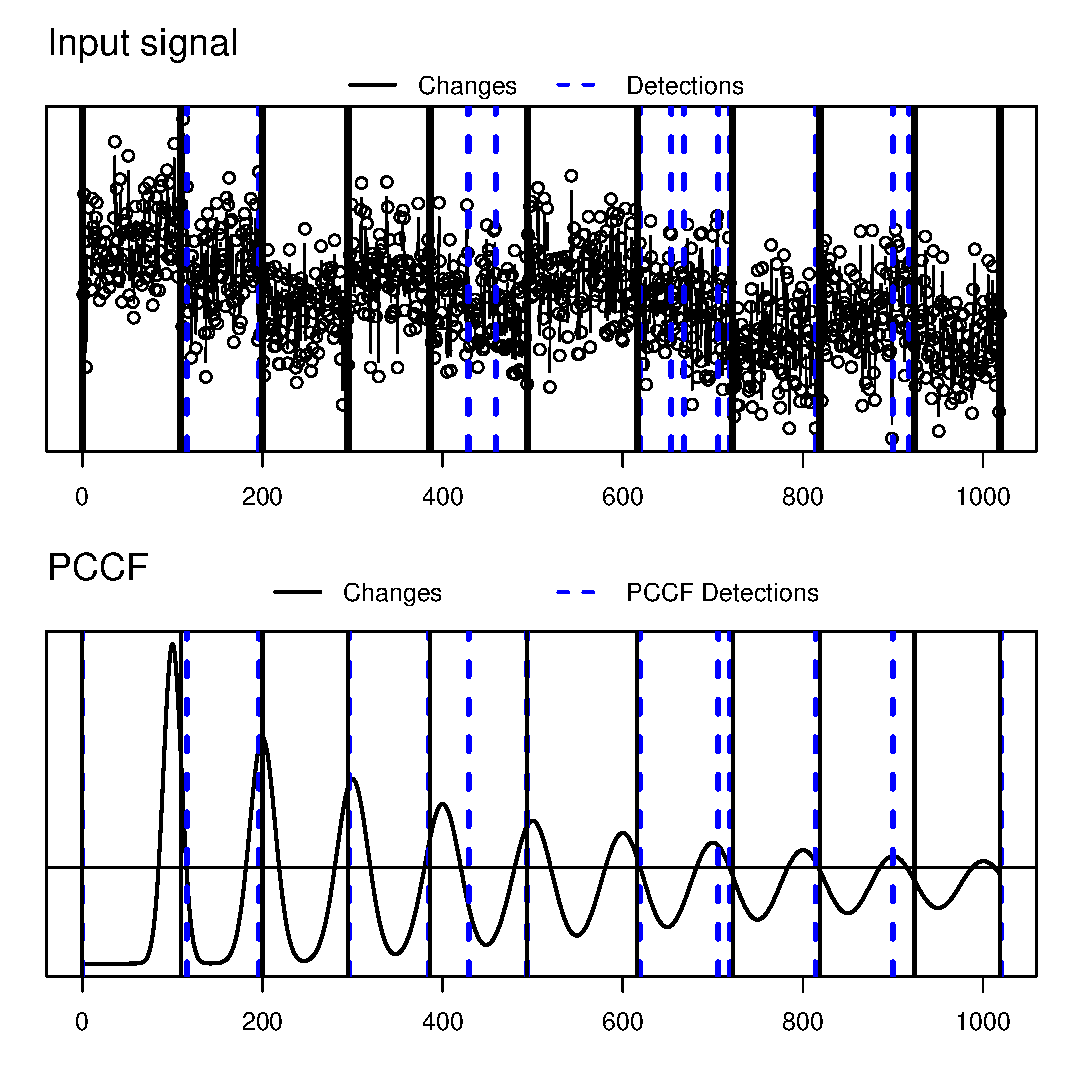
\includegraphics[width=0.8 \textwidth,
            trim={0.5cm 0cm 0.5cm 0cm}]{./images/blpa_article/fig3_concept_proof.eps}}
        \fbox{\includegraphics[
            width=0.787\textwidth,
            height = 0.27 \textheight,
            trim={0.0cm 1cm 1cm 1.7cm}]{./images/blpa_article/sim1_roc.eps}
            }
        \caption{
            Experimental results for simulated data streams with recurrent changes.
            On the top plot - an example of the generated input signal.
            %
            Vertical solid lines depict changepoints to be detected. 
            Dashed lines on the plot with the signal depict moments when detector \textbf{without} PCCF alarmed changes.
            %
            Bottom plot - ROC curves. 
            Blue triangles depict performance of the detector equipped with PCCF.
            Black dots - performance without PCCF.
            FP rate is reduced while keeping the same TP rate.
            }
            \label{fig:results1}
    \end{minipage}
\end{figure}
FP rate is decreased while not reducing TP rate.
In the worst cases the performance of both detectors is similar.

\subsection{Human Activity (HA) signal}
%https://archive.ics.uci.edu/ml/datasets/Smartphone-Based+Recognition+of+Human+Activities+and+Postural+Transitions
In the second experiment we used the Human activity data set~\cite{reyes2016transition} which contains sensor measurements from people performed 6 types of activities: three static postures (standing, sitting, lying) and three dynamic activities (walking, walking downstairs and walking
upstairs).
We detected changes in the signal caused by transitions from one set activities to another.
Results are depicted in Fig.~\ref{fig:results2}.
\begin{figure}[!htb]
%this is \input{FigResults2.tex}
    \begin{minipage}{0.5\textwidth}
        \centering
        \fbox{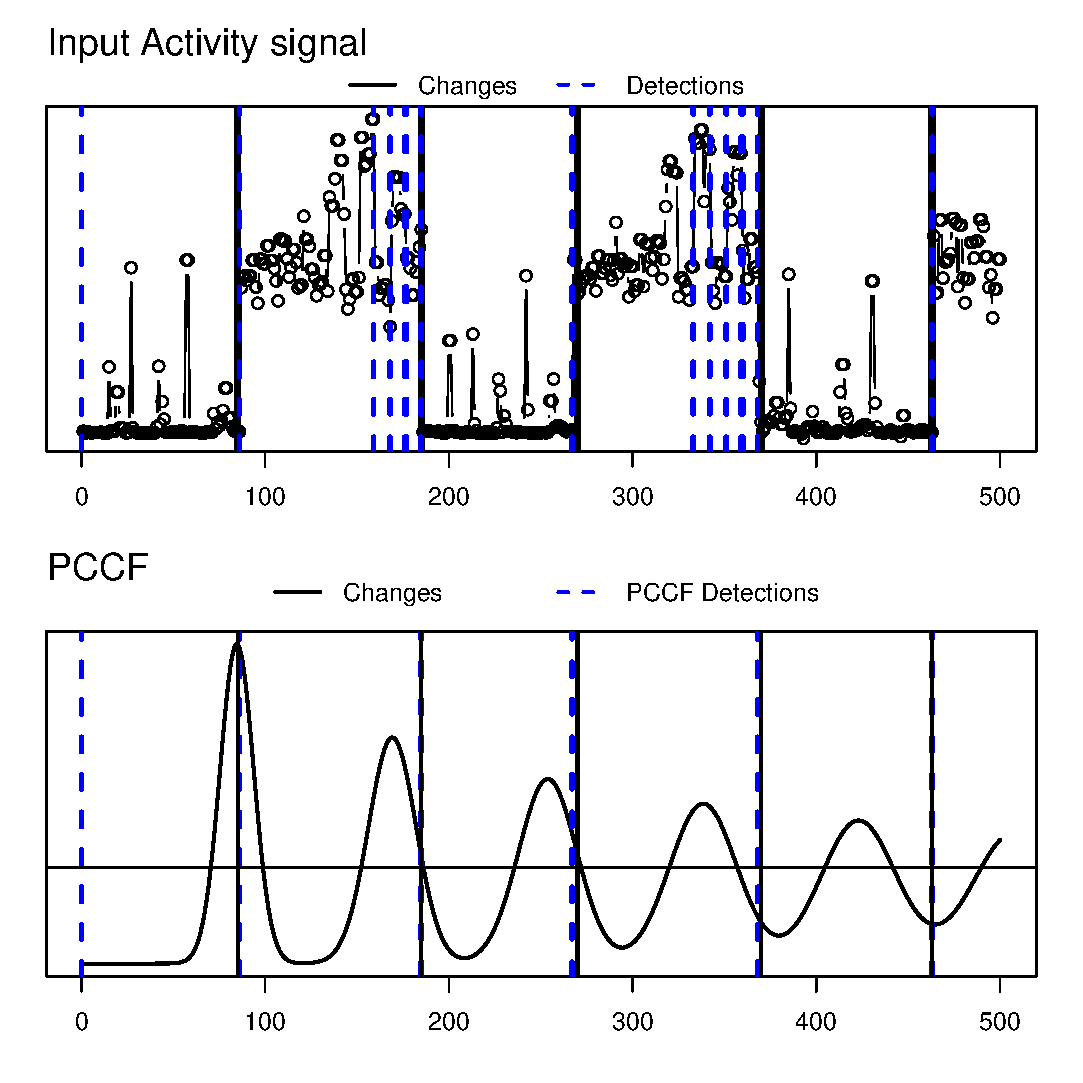
\includegraphics[width=0.8\textwidth, trim={0.5cm 0cm 0.5cm 0cm}]{./images/blpa_article/fig4_concept_proof_real.eps}}
        \\
        \fbox{
            \includegraphics[
            width=0.773\textwidth, 
            height = 0.27 \textheight,
            trim={0.0cm 1cm 1cm 1.7cm}]{./images/blpa_article/exp1_roc_real.eps}
            }
        \caption{
         Experimental results for the 'Activity recognition' signal.
         On the top plot - illustrating example of the signal and corresponding PCCF function.
         Vertical solid lines depict changepoints to be detected. 
         Dashed lines on the plot with the signal depict moments when detector \textbf{without} PCCF alarmed changes. 
         Dashed lines on the plot \textbf{with} PCCF show time moments when the detector with PCCF alarmed changes.
         Bottom plot - ROC curves. 
        Blue triangles - performance of the BD with PCCF.
            }
            \label{fig:results2}
    \end{minipage}
\end{figure}
FP rate is decreased when BD detector is used with the PCCF function.

\section{From Journal: Integration with CuSum}

\subsection{Cumulative Sum (CuSum) detector}~\label{subsec:cusum_detector}
In this section, we describe the CuSum~\cite{Page1954} detector and its output statistic properties important for measuring performance metrics in static and dynamic settings.
Changes in the stream of measurements reflect dynamics of observed phenomenon happening in time.
Therefore, strictly speaking, any change is a gradual process.
In this paper, for simplicity, we refer to change points and to detections as individual time moments as if change would have happen instantly. If change is gradual and spans time interval then it can be reduced to a single time moment by considering the start or end of the change event~\footnote{Gradual change may become represented as an abrupt change in the time series also due to the sampling rate of measurements}. 
Change points in the signal are characterized by the time moment when they happened and by the corresponding mean shift value in the signal.
\begin{definition}
  Change point is a time moment $t^c$ when statistical properties of the data stream change significantly accordingly to a predefined criteria.
\end{definition}
\begin{definition}
  Detection is a time moment $t^d$ when a detector alarms a change.
\end{definition}
For example, if $x_i \sim \mathbb{N}(\mu_1, \sigma)$ for $i < k$ and $x_i \sim \mathbb{N}(\mu_2, \sigma)$ for $i \geq k$,
then we say that a change point occurred at time moment $t_k$, i.e. $t^{\text{c}}_{k} \equiv t_k$.
In general, detection can usually be alarmed before or after a change point.
If $t^{\text{d}}_k > t^{\text{c}}_k$, then change is detected with the delay $t^{\text{d}}_k - t^{\text{c}}_k$.
If $t^{\text{d}}_k < t^{\text{c}}_k$ then detection $t^{\text{d}}_k$ is a false alarm (FA).

As an input, CuSum detector receives time series of observations~\ref{eq:input_ts} usually taken at constant sampling rate.
\begin{equation}\label{eq:input_ts}
	(x_i)_{i=1}^{N} \equiv (x_1, x_2, \dots, x_N)
\end{equation}
taken at corresponding time moments $(t_i)_{i=1}^N$.
Observations and time moments are enumerated by index $i$ mapping $t_i$ to observations $x_i$ and vice versa.
CuSum works through a sequential calculation of the output statistic as follows
% Cusum rule: https://www.itl.nist.gov/div898/handbook/pmc/section3/pmc323.htm
\begin{align}
	S_0 &= 0 \nonumber \\
	S_{n} &= \max (0, S_{n-1} + x_n - \mu_0 - k )\label{eq:cusum_scheme}.
\end{align}
Detections are alarmed at time moments when $S_{t+1} > h$, i.e. when output statistic exceeds a threshold value $h$.
In \eqref{eq:cusum_scheme}, $\mu_0$ is the estimate of the in-control state signals' mean value.
The parameter $k$ is called allowance value and it depends on the level of mean shift $\delta=\mu_2-\mu_1$ that we aim to detect.
Notations used throughout the article are summarized in Table~\ref{tab:notations}. Table~\ref{tab:interchangeable} summarises terms which we use interchangeably.
\begin{table}[!htb]
	\begin{tabular}{|l|l|}
		\hline\noalign{\smallskip}
		Index to enumerate observations and time moments & $i$ \\
		Index to enumerate changes and detections & $k$ \\
		Input signal & $(x_i)_{i=1}^{N} $ \\
		Time moments & $(t_i)_{i=1}^{N}$ \\
    Change points & $t_{k}^{\text{c}}$ \\
		Detections & $t_{k}^{\text{d}}$ so that  $t_{k}^{\text{c}} \in (t_i)_{i=1}^{N}$ and  $t_{k}^{\text{d}} \in (t_i)_{i=1}^{N}$   \\
		Detection delay & $t_k^{\text{d}} - t_k^{\text{c}}$ \\
		Signal mean values before and after change& $\mu_1$, $\mu_2$ \\
		Mean shift & $\delta=\mu_2 - \mu_1$   \\
		Threshold for Cusum output statistic & $h$  \\
		Average run length given $\delta$ & $ARL_{\delta}$ \\
		Average run length given $h$ & $ARL_{h}$ \\
		Width of the prediction interval (ROI) & $\text{ROI}_{\text{Width}}$  \\
    Binary performance metrics (Number of corresponding events) & TP, FA, FN \\
		\noalign{\smallskip}\hline
	\end{tabular}
	\caption{Notations summary}~\label{tab:notations}
\end{table}
\begin{table}[!htb]
	\begin{tabular}{| l | l |}
		\hline\noalign{\smallskip}
    Prediction intervals & ROI (Region Of Interest) \\
    Dynamic/Static settings detector & Detector using / not using prediction intervals \\
    Detection threshold $h$  & Detector's sensitivity $h^-1$ \\
		\noalign{\smallskip}\hline
	\end{tabular}
	\caption{Abbreviations and interchangeable terms}~\label{tab:interchangeable}
\end{table}

\subsection{ARL}
The key performance metric of the CuSum detector is the Average Run Length (ARL), which refers to the expected number of observations before an action is taken, i.e., before the detection is alarmed~\cite{Page1954}.
ARL refers to the FA rate before the change and to the detection delay after the change point.
When the process is in-control, the $ARL_{\delta}$ refers to a FA rate, whereas when the change has happened it refers to the detection delay.
However, ARL is hard to estimate analytically.
As reported in~\cite{plasse2021streaming}, one of the simplest ARL approximations is given in~\cite{siegmund2013sequential} in a form of the following equation 
\begin{equation}\label{eq:arl_approximation}
	\text{ARL}_{\delta} = \frac{\exp(-2(\delta-k)h') + 2(\delta - k)h' -1}{2 (\delta - k)^2}
\end{equation}
for $h' = h+1.166$.
Figure~\ref{fig:arl} depicts ARL behavior against $\delta$ (left plot) and versus threshold $h$ (right plot).
It is easy to see how ARL refers to both the FA rate and to the detection delay at the same time.
More precisely, smaller values of $\delta$ correspond to fluctuations in the signal and to the larger ARL values, whereas
larger values of $\delta$ indicate change points to be detected.
Not surprisingly, ARL decreases fast when $\delta$ is increased.
It also can be seen that by changeing $\delta$ we increase or decrease ARL value.
We will use this fact later in the experimental part when performing simulations to measure the detection delay by varying ARL values (by changing $\mu_2-\mu_1 \equiv \delta$) for static and dynamic detectors.
%
\begin{figure}[!htb]
	\centering
	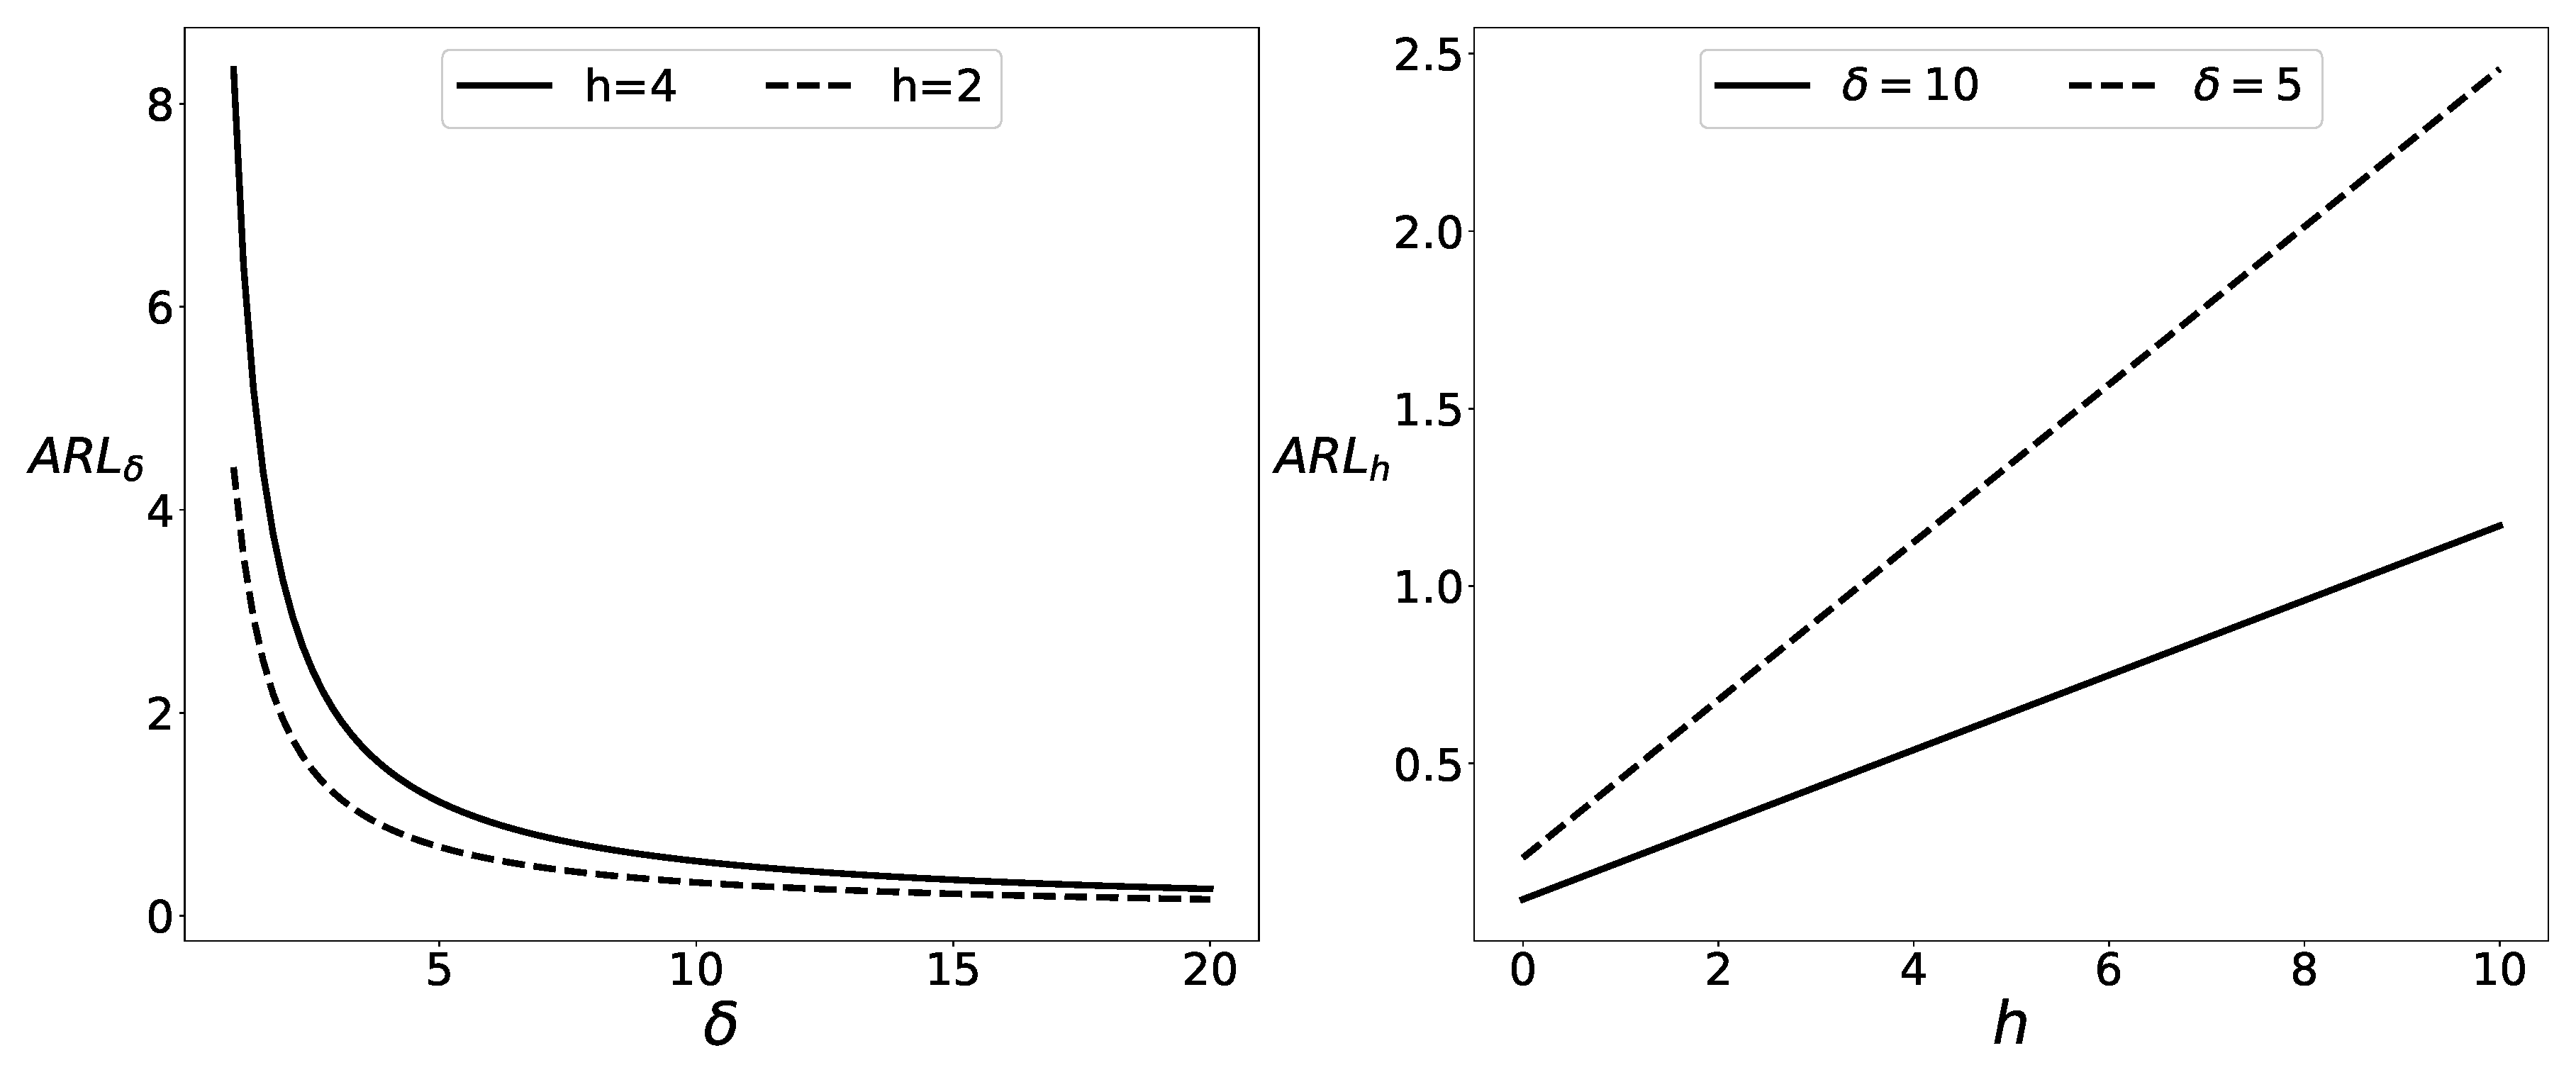
\includegraphics[width=0.9\textwidth]{articles/pics/journal_paper/arl.eps}
	\caption{
    The left plot depicts ARL as a function of $\delta = \mu_2-\mu_1$ for two fixed threshold values $h$. The right plot depicts ARL as a function of the threshold value $h$ for two fixed $\delta$ values (Equation~\ref{eq:arl_approximation}).
    Both plots demonstrate that smaller ARL values (and therefore detection delays) correspond to smaller $h$ values. It is obvious for the right plot, on the left plot this fact is depicted by the dashed line for $h=2$ being lower than the solid line for $h=4$.
    %
    Smaller $\delta$ corresponds to the fluctuations in the time series causing false alarms, larger $\delta$ correspond to changes in the level shift which are subject for detection.
    When threshold $h$ is adjusted to smaller values ARL for all $\delta$ values gets smaller (left plot), therefore detection delay is decreased but probability of FA is increased.
}\label{fig:arl}
\end{figure}

\subsection{Random walk property of CuSum output statistic}
In order to investigate how detection delay and false alarm rate depend on the detection threshold $h$ in static and dynamic settings, it is important to describe CuSum's statistical properties before and after a change point.
Assuming that the input signal before the change follows
$x_i \sim \mathbb{N}(\mu_0, \sigma)$
and after the change
$x_i \sim \mathbb{N}(\mu_0 + \delta, \sigma)$, the
CuSum's output statistic can be calculated as
$s_i = x_i - \mu_0$ if $i == 0$,
and as
$s_i = s_{i-1} + x_i - \mu_0$ if $i > 0$.
%
If $x_i \sim \mathbb{N}(\mu_0, \sigma)$ then
$x_i - \mu_0 \sim \mathbb{N}(\mu=0, \sigma)$
before the change, and, therefore, the CuSum's statistic
$s_i =s_{i-1} + x_i - \mu_0$ is a Gaussian random walk
$s_i = \sum_{i=0}^{k} (x_i \sim \mathbb{N}(\mu=0, \sigma))$.
Furthermore, after the change,
$x_i - \mu_0 \sim \mathbb{N}(\delta, \sigma)$
and, therefore, $s_i$ is a random walk with the drift.
%
So, before the change CuSum's output statistic behaves as a Gaussian random walk (RW) stochastic process and after the change as a random walk with the drift (see example on Figure~\ref{fig:possible_outcomes}).
Variance of the RW increases over time as a function of $\sigma \sqrt{t}$ with expected value staying around $0$.
Expected value of the RW with drift increases according to the linear trend $\sim t \mu$.
That is why ARL increases as it is depicted on the right plot of Figure~\ref{fig:arl} with increasing threshold value $h$ according to the Equation~\ref{eq:arl_approximation}.
It also becomes clear that false alarm events are caused not only by input signal properties but also by the stochastic nature of the CuSum's output statistic.
Even if there is no change point in the signal, there is still a non-zero probability of FA event.
This is depicted on the left plot in Figure~\ref{fig:arl} by large values of ARL corresponding to small values of $\delta$.

Let us comment Figure~\ref{fig:possible_outcomes} depicting Cusum's output statistic before and after a change point.
Figure depicts two detections, change point location in the middle, threshold value (horizontal line), and prediction intervals (ROI).
Depicted threshold value is not optimal on a global scale for the whole signal, but it is optimal locally in case if we use a prediction interval.
In this case the first detection, which is a false alarm, is skipped, while second detection is a correct detection with a smaller detection delay in comparison to the case where we would use larger $h$ on the global scale in order to skip false alarms.
This example demonstrates that despite the fact that by making threshold value smaller we decrease ARL values both for detection delay and for false alarms, according to the Figure~\ref{fig:arl} and Equation~\ref{eq:arl_approximation}, it is still possible to improve the performance both for detection delay and FA rate.
Smaller ARL imply higher probability of false alarms but number of false alarms can be lower in dynamic settings, because we consider subsets of the input signal which are within prediction intervals.
Plots in column B on Figure~\ref{fig:possible_outcomes} illustrates the opposite case when the performance is decreased when using the prediction interval (ROI).
Run length for detection after a change point happens to be longer than the ROI width. Other outcomes are possible which are discussed in detail in the Section~\ref{sec:performance} about performance metrics.

An important factor to note is that if we wouldn't have strict constraints on the detection delay to be that small as depicted on Figure~\ref{fig:possible_outcomes}, then the optimal strategy would be to just increase threshold value and it would result in zero FA rate and in a longer detection delay.
So, we consider optimality of change detection in the presence of prediction intervals when having constraints on the detection delay values.
\begin{figure}[!htb]
	\begin{minipage}[t]{1.0\textwidth}
    \centering
    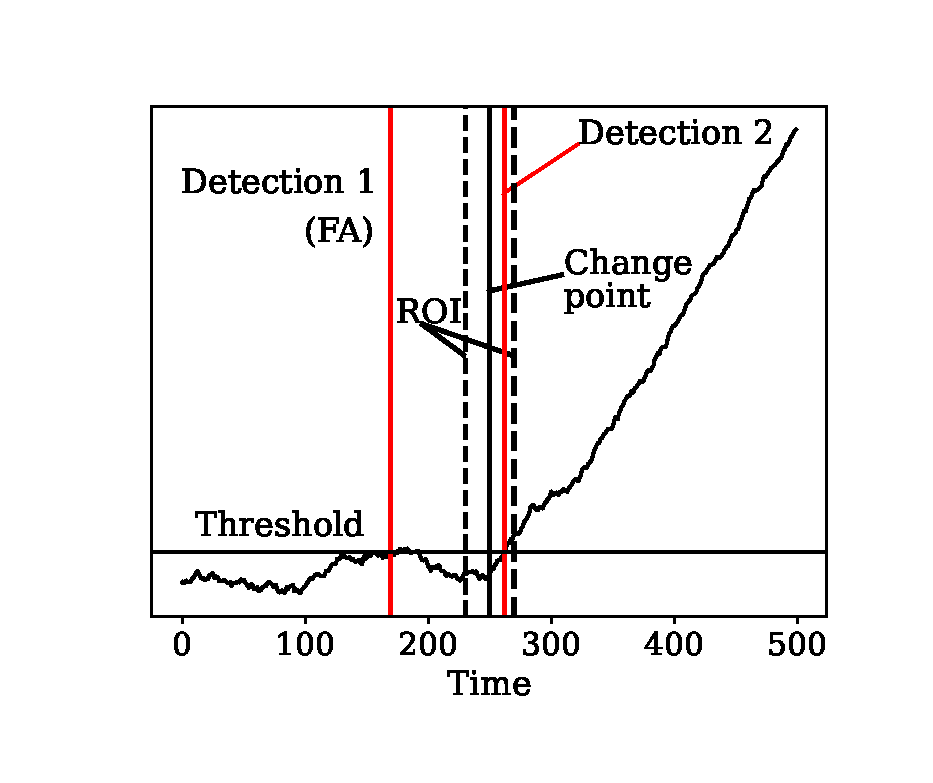
\includegraphics[width=0.44\textwidth, trim={1.5cm 1.0cm 0.3cm 1.0cm}]{articles/pics/journal_paper/proof_of_concept2.eps}
    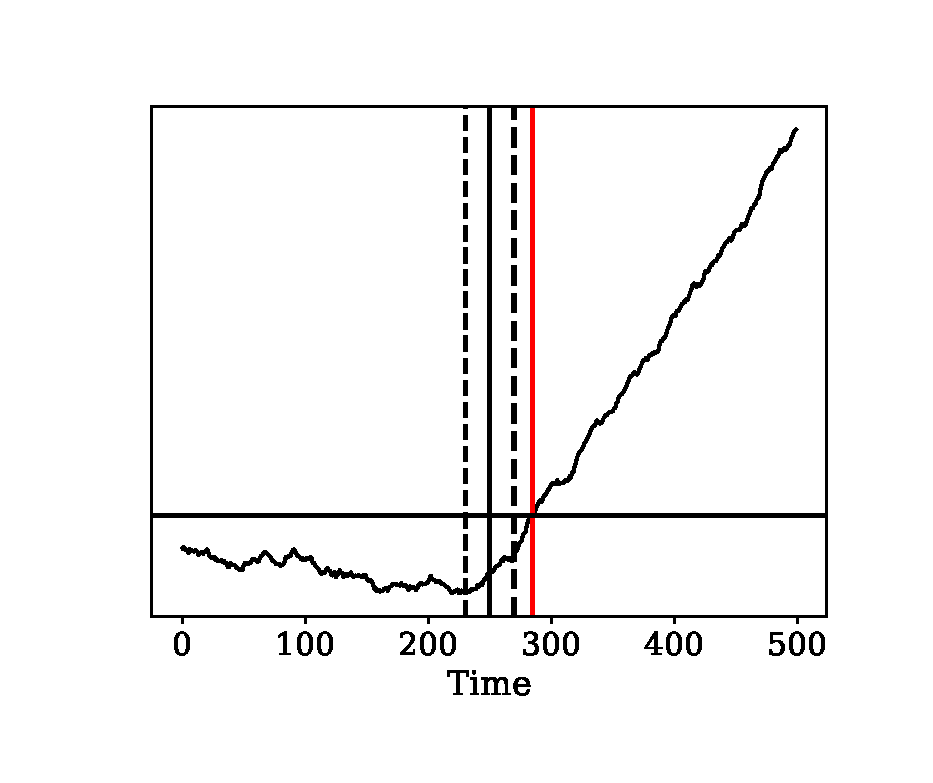
\includegraphics[width=0.44\textwidth, trim={1.5cm 1.0cm 0.3cm 1.0cm}]{articles/pics/journal_paper/proof_of_concept2_fn_case.eps}
    \\
		\includestandalone[width=0.35\textwidth]{articles/pics/journal_paper/tikz/perf_metrics_case1}
    \hspace{10mm}
		\includestandalone[width=0.35\textwidth]{articles/pics/journal_paper/tikz/perf_metrics_case2}
		\caption{
    Left side plots depict how performance can be improved with prediction interval (ROI). 
    Detection 1 is false alarm and it is ignored since it is outside ROI. 
    Detection 2 is alarmed after the change point with a small delay. 
    Without ROI we would have to increase threshold in order to avoid FA, but in this case detection delay would increase.
    Right side plots depict the case when performance is decreased when using prediction. Prediction interval is correct but the width of the interval isn't enough to detect change within it what leads to FN event. 
    Plots at the bottom depict how performance metrics are calculated.
    In both cases FA event causes FN event.
    If detection happens after the change but outside ROI (right side) then it is counted as FA.
    }~\label{fig:possible_outcomes}
	\end{minipage}
\end{figure}


\subsection{Performance metrics}~\label{sec:performance}
As mentioned in Section~\ref{sec:cusum_detector}, the commonly used change detection performance metric with Cusum is the ARL value, which refers to the FA rate before change point and to the detection delay after the change.
In case of multiple change points, the ARL metric is not sufficient as it doesn't reflect how many changes were detected and missed.
As in~\cite{bodenham2017continuous} and in~\cite{plasse2021streaming}, in addition to the detection delay, we use binary classification metrics to assess performance of the change detection process.
We define those metrics in terms of mappings between change and detection events as follows.
\begin{definition}
	We define TP, FA, FN and TN events in terms of mappings between change points and detections.
	To every TP corresponds one change point.
	FA is the detection to which there is no any corresponding change point.
	FN is change point to which there is no corresponding detection.
	More formally
	\begin{itemize}
    \item \textit{TP is a first detection (DE) after change point.} E.g., if $\text{changes}=[100], \text{DEs}=[50, 110, 121]$ then TP is $\text{d} =110$.

    \item \textit{Detection delay is a time interval between TP and corresponding change point} $t_{\text{d}} - t_{\text{c}} \geq 0$. If detection doesn't happen $\text{NaN}$ value is assigned to the delay.

    \item \textit{FA is a detection before change point or detection after another detection which was TP but before next change point.} E.g., if $\text{changes}=[100], \text{DEs}=[50, 110, 121]$ then FA are $\text{DEs} = [50, 121]$.

    \item \textit{FN is an event when there is no detection corresponding to the change point.} E.g., if $\text{changes}=[100, 150], \text{DEs}=[50, 110, 121]$ then FN is $[150]$. FN can be caused by events 1) Cusum output statistic didn't exceed threshold $h$ 2) in the dynamic case - if DE was alarmed after change point but not within prediction interval. E.g., if $\text{changes}=[100], \text{DEs}=[50, 121]$, prediction interval is $\text{ROI}=[(90, 110)]$ then FN is change point $[100]$.

    \item \textit{TN is every event when detection is not alarmed correctly}, i.e. - if alarmed it would cause FA.

\end{itemize}
\end{definition}
Figure~\ref{fig:possible_outcomes} illustrates given definitions for static and dynamic settings. As in~\cite{plasse2021streaming} we use $F_1=\frac{TP}{TP+\frac{1}{2}(FA+FN)}$ score metric combining precision and recall to measure detection performance along with the detection delay value.
There is a similarity to binary classification but analogy is not full because any change in real signal takes time.
And therefore all time moments and observations within change time interval should be labelled as change.
During change detection using CuSum no labels to observations or time moments are assigned.
CuSum alarms detection when its output statistic exceeds threshold.


\subsection{Experiments}\label{sec:experiments}
We perform two experiments to show how CuSum detection performance can be improved with prediction intervals. 

\subsubsection{Implementation}\label{sec:implementation}
Before the experimental results, we describe how the combination of Pccf in Section~\ref{sec:pccf} and the CuSum detector in Equations~\ref{eq:cusum_scheme} is translated to a change point detection framework.
The implementation is depicted in Algorithm~\ref{alg:method_code}.
The core logical part is a code snippet:
\begin{algorithm}[!h]
	\begin{algorithmic}
    \If{(not PCCF) or (PCCF and WithinRoi()) }
        \If{$|stat[t]| > h$}
            \State detections.append(t)
            \State ResetDetector()
        \EndIf
    \EndIf
	\end{algorithmic}
\end{algorithm}

\noindent
which states that the CuSum stopping rule is checked continuously if no prediction intervals (ROIs) are provided or checked only within ROI intervals if they are available. If so, the detection is collected to the array  and detector's settings are re-initialized. In case of a sequential change detection a new in-control mean value of the input signal is estimated using function $UpdateMu$ after each detection. An important property of the implementation is that  when detection happens before change point or does not happen at all then detection delay has NaN value (lines 17-18, Algorithm~\ref{alg:method_code}). And delay mean value is calculated after removing NaN values.


\subsubsection{Artificial signal simulation}
In the first experiment we perform a simulation to measure average values of the detection delay and $F_1$ score of the CuSum detector in the presence of prediction interval and without it. We will measure performance while variating detection threshold $h$ and level shift in the mean value $\delta=\mu_2-\mu_1$, controlling signal-to-noise ratio. These two parameters are controlling ARL value (Figure~\ref{fig:arl}, Equation~\ref{eq:arl_approximation}).
We expect to see performance gain in dynamic case for small $h$ values when corresponding ARL is smaller or equal to the $\text{ROI}_{\text{Width}}$. For larger $h$ values detection will happen outside ROI (Figure~\ref{fig:possible_outcomes}) and static detector should perform better. 

Input signal was generated $1000$ times by drawing samples from Gaussian distribution with parameters $\mu_1=0, \sigma=1$ before change at time moment $t^c = 100$ and $\mu_2 \in [1.1, 2.1, 3.1], \sigma=1$ after change.
Prediction interval of width $\text{ROI}_{\text{Width}}=50$ is located in the middle of the signal symmetrically to the changepoint.
Performance metrics are measured while changing detection threshold value $h$ and signal level shift $\delta$.
Level shift $\delta$ is being increased in order to decrease corresponding ARL (Figure~\ref{fig:arl}, Equation~\ref{eq:arl_approximation}) and its ratio to the $\text{ROI}_{\text{Width}}$.
When ARL becomes larger we expect to see less performance gain when using dynamic settings since static detector will be able to detect change with similar delay.

Figure~\ref{fig:artificial_signal_perf_results} depicts the results.
Plots on the left side show averaged detection delays.
Plots on the right side show averaged $F_1$ score values.
Three rows of plots from top to down depict cases for different $\delta$ values.
Both in case of dynamic and static detector settings, when $h$ is small the detection delay is also small but there are a lot of false alarms. 
When threshold increases $F_1$ score increases because of fewer FA and the detection delay gets bigger. 

Detection delay with prediction interval is lower or the same as in case without prediction interval for all $h$.
Dashed curve depicting dynamic detector delays is shorter that solid curve corresponding to the static detector because because dynamic detection delay can't exceed half of the $\text{ROI}_{\text{Width}}$ (since ROI is symmetrical to change point location). 
In case of FA event detection delay is assigned to $\text{NaN}$ value. 
While calculating average value $\text{NaN}$ values are ignored. 
Therefore detection delay plot depicts only successful detections cases. 
The cases when delay is $\text{NaN}$ are captured by FA and FN factors in $F_1$ score value.

Dynamic CuSum $F_1$ score outperforms static CuSum (Figure ~\ref{fig:artificial_signal_perf_results}) for smaller $h$ values when false alarms outside ROI are skipped and change is detected within ROI. 
This situation is depicted on the left side of Figure~\ref{fig:possible_outcomes}.
When $h$ increases CuSum ARL exceeds $\text{ROI}_{\text{Width}}$ and detection doesn't happen within ROI.
This is depicted on the right side of Figure~\ref{fig:possible_outcomes}. 
\begin{figure}[!htb]
	\centering
	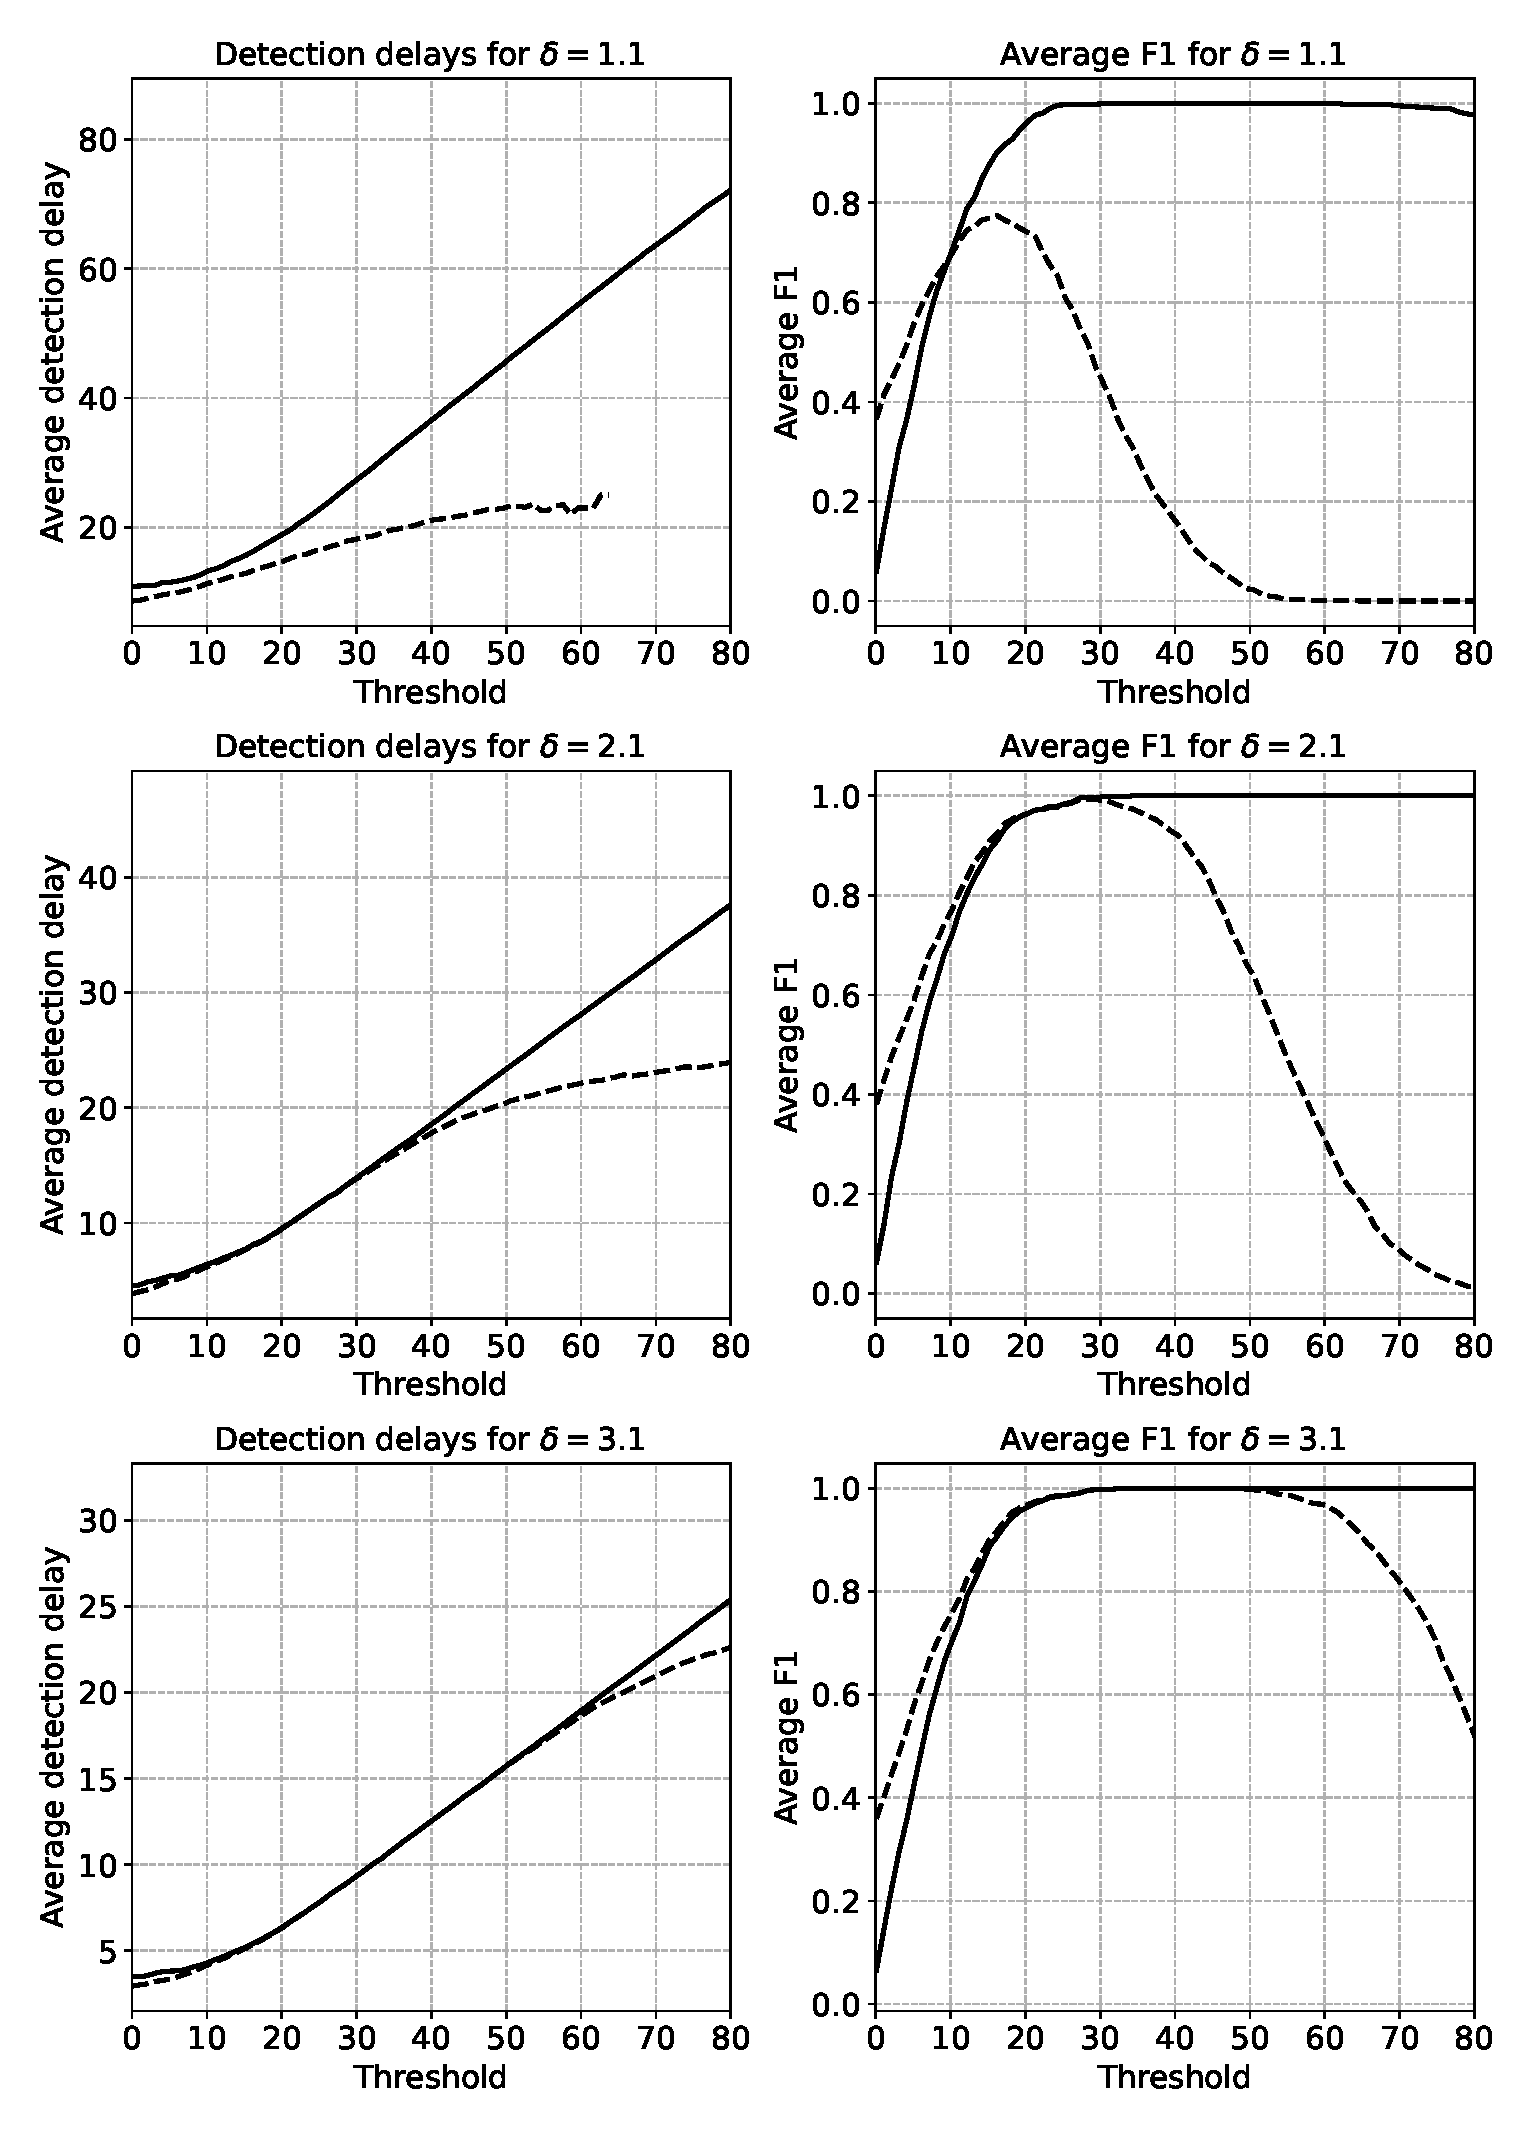
\includegraphics[width=0.90\textwidth]{articles/pics/journal_paper/performance_detection_sim}
	\caption{Average detection delays (left side) and average $F_1$ score (right side) when variating threshold value $h$ (x-axis).
	Top, middle and bottom rows of plots are for different $\delta = \mu_2 - \mu_1$ values.
	Solid and dashed lines depict static and dynamic cases.
    Average delay is calculated after ignoring NaN values caused by FA.
    NaN delay values and corresponding FA events are counted by $F_1$.
    For small $h$ values corresponding to smaller ARL values comparable to the prediction interval width, dynamic CuSum performance is better.
    When $h$ gets larger static detector $F_1$ score starts exceeding dynamic detector curve.
    Detection delay plots depict only cases when FA event didn't happen, therefore it should be analyzed along with $F_1$ metric.
    Dynamic CuSum has better performance with the given ROI for $h$ values when $F_1$ dashed curve (dynamic case) is above solid curve (static case).
	}
	\label{fig:artificial_signal_perf_results}
\end{figure}


\subsubsection{Temperature data}
In the second experiment, we predict and detect multiple change points in the time series of temperature measurements collected from the sensor installed in the home office environment.
We measure the same performance metrics, except ARL, as in the first experiment when trying to predict all changes using Pccf and when predicting only several most earliest change points.
In the second experiment, we confirm results obtained in the first experiment using the real signal and, in addition, we investigate sensitivity of the results with regard to the prediction accuracy when calculating prediction intervals using Pccf.
An important difference also is that in this experiment we do not average detection delay values and therefore we also compare detection delays in static and dynamic cases directly without possibility to disregard $NaN$ values due to averaging.
Measurements took place in the city of Jyv\"{a}skyl\"{a} (Finland) from 06 Mar 2021 (19:11m) until 21 Mar 2021 what is a cold period in Finland.
Subject for the change detection is the beginning of every working day when heater was turned on in the morning and what caused abrupt changes in the ambient temperature.
Figure~\ref{fig:dht22} illustrates the measuring device.
\begin{figure}[htb!]
	\centering
	\includegraphics[width=0.4\textwidth]{articles/pics/journal_paper/DHT22.png}
	\caption{
		Arduino Uno board with attached DHT22 temperature and humidity sensor.
		When it was not cloudy the sun light shined directly on the sensor through the window in the noon causing temperature peaks.
	}
	\label{fig:dht22}
\end{figure}
Temperature measurements were taken 1 time per 60 seconds using DHT22 temperature and humidity sensor connected to the Arduino board.
Figure~\ref{fig:temperature_signal} illustrates temperature signal.
Figure~\ref{fig:performance_temperature_signal} illustrates results.
\begin{figure}[!htb]
	\centering
	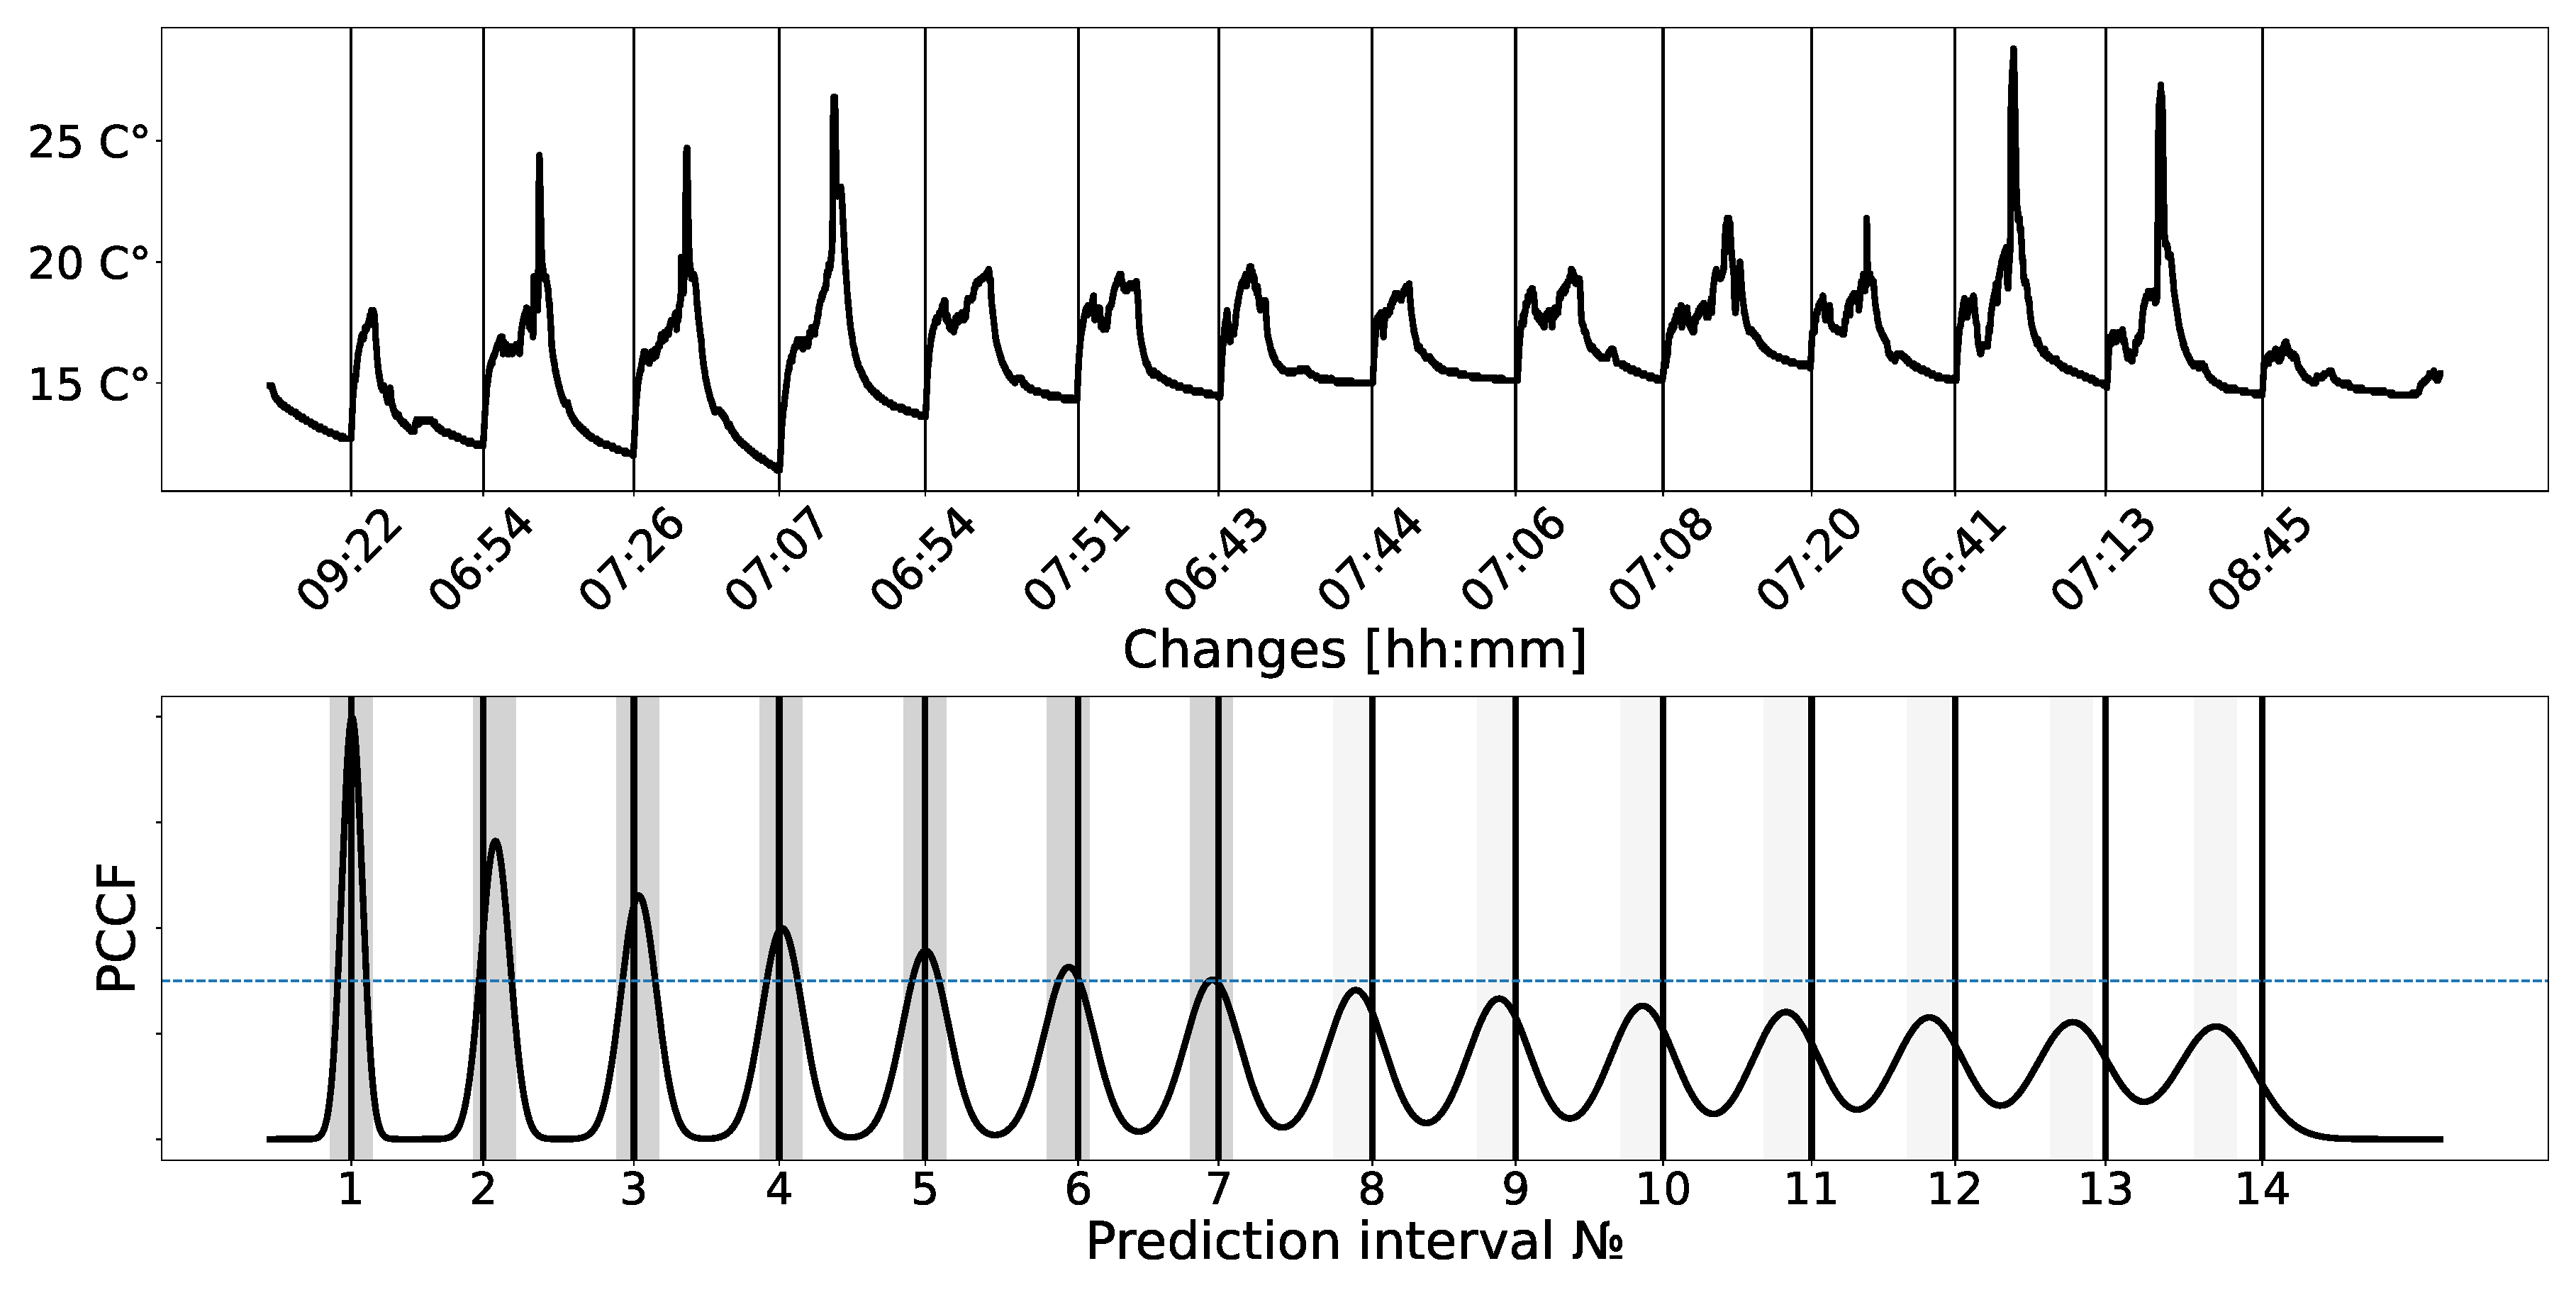
\includegraphics[width=0.9\textwidth]{articles/pics/journal_paper/temperature_signal}
	\caption{
    Temperature signal and Pccf.
    Changes are depicted by vertical solid lines on both plots.
    Prediction intervals are enumerated and marked by grey vertical regions on the bottom plot. First 7 changes are predicted with a good accuracy, further change points are not within prediction intervals.
  }
	\label{fig:temperature_signal}
\end{figure}
\begin{figure}[!htb]
		\centering
  \begin{tikzpicture}[scale=0.9]
		\draw(0, 0) node{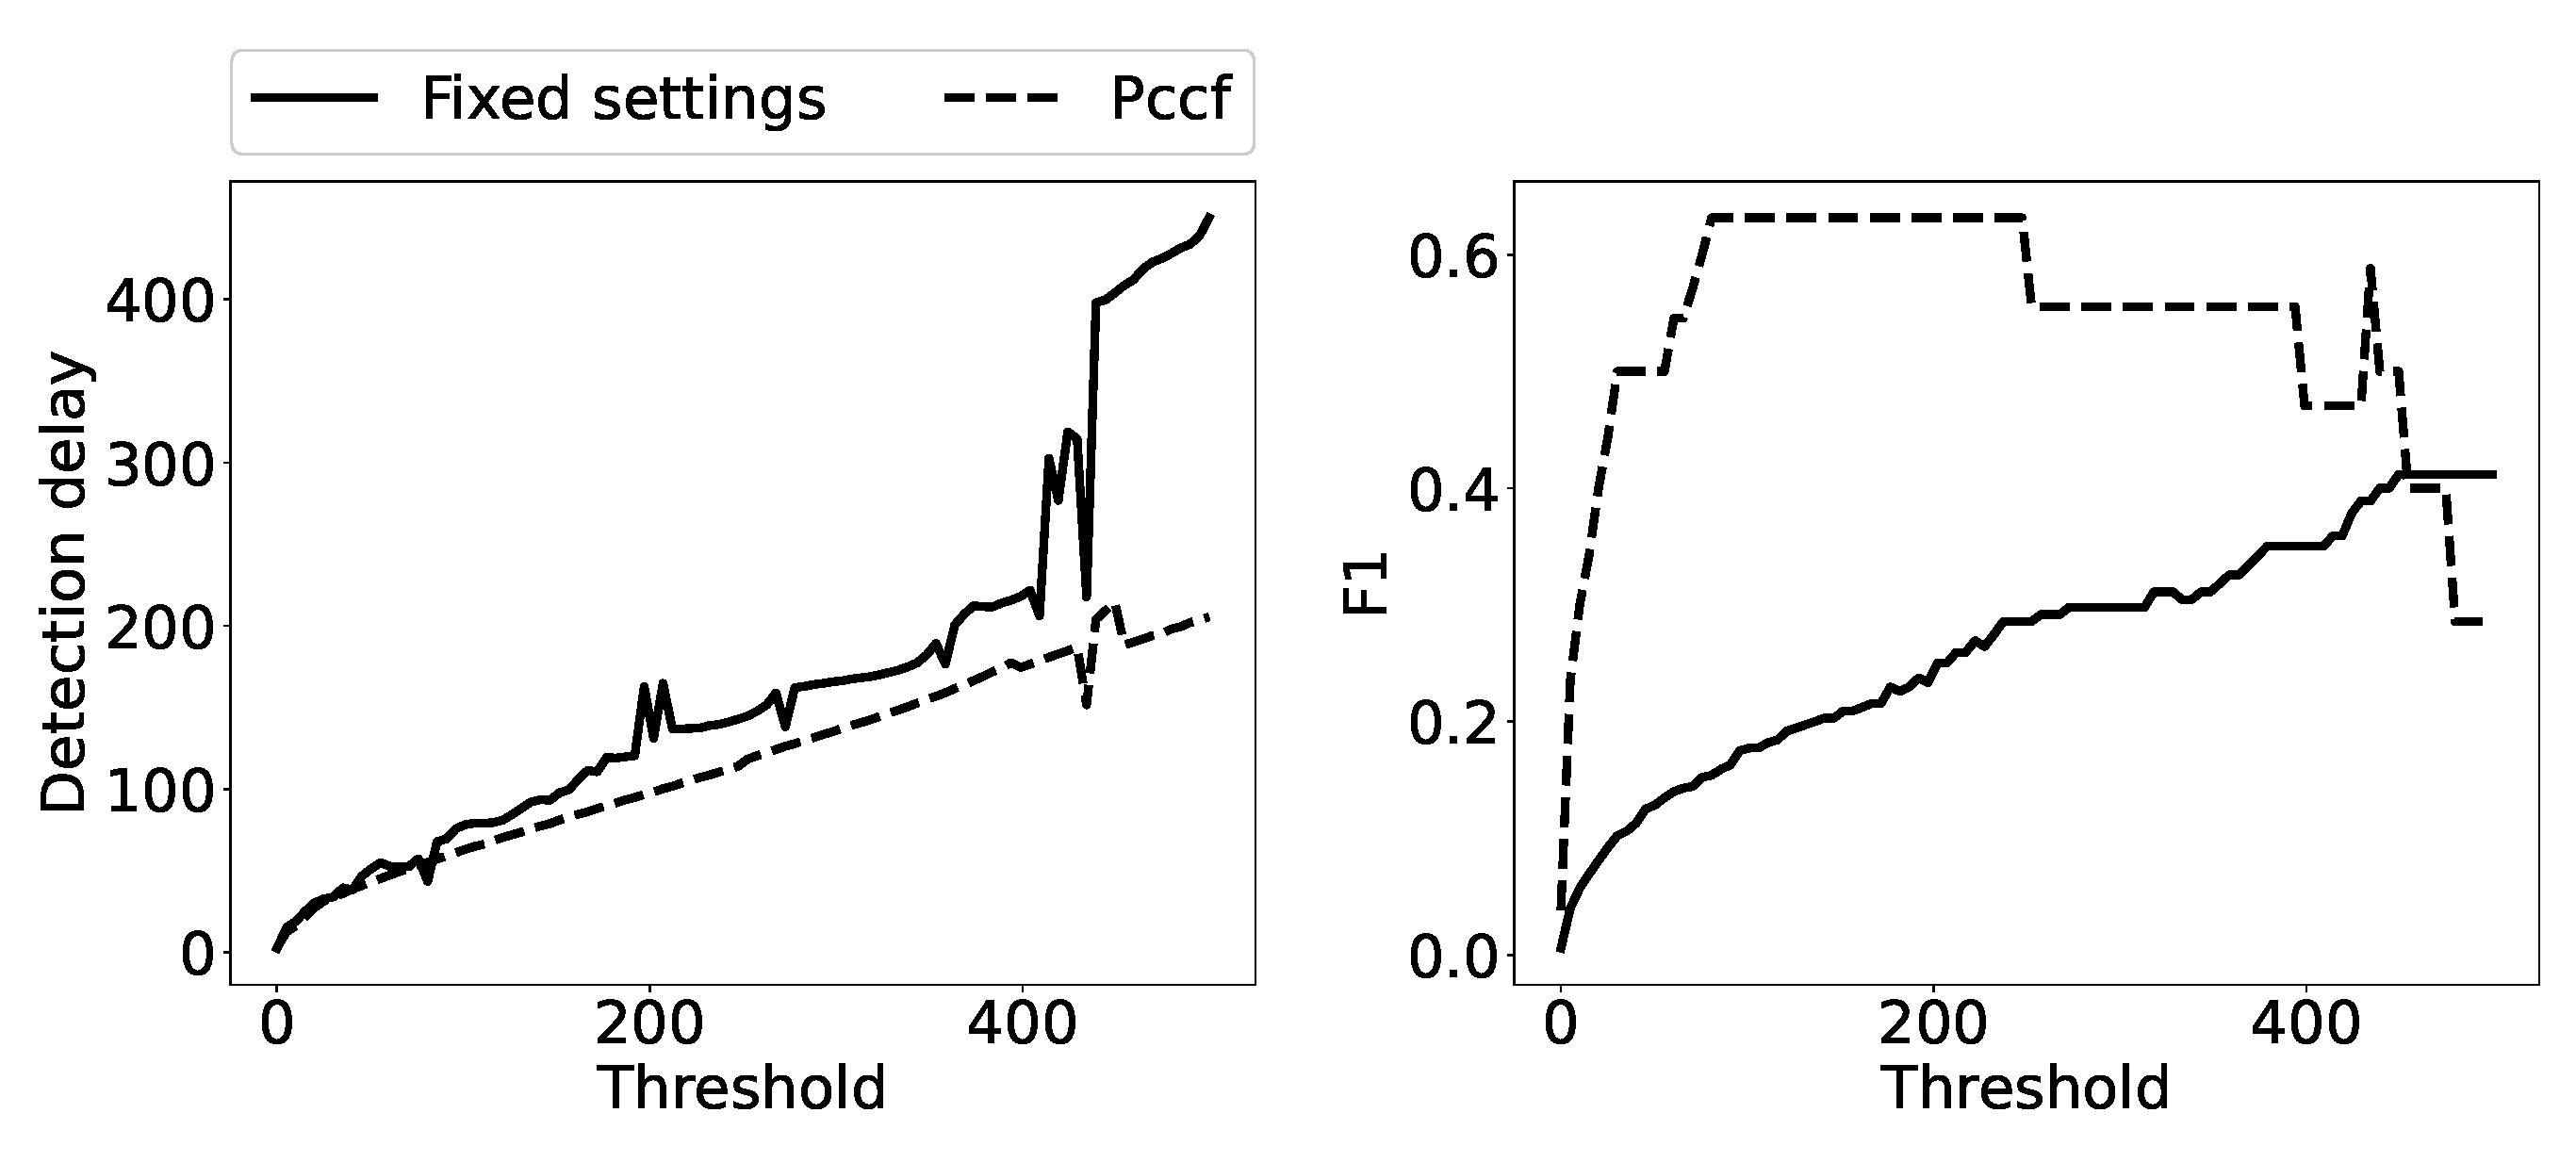
\includegraphics[width=0.8\textwidth]{articles/pics/journal_paper/performance_temperature_seven}};
		\draw(0, -4.8) node{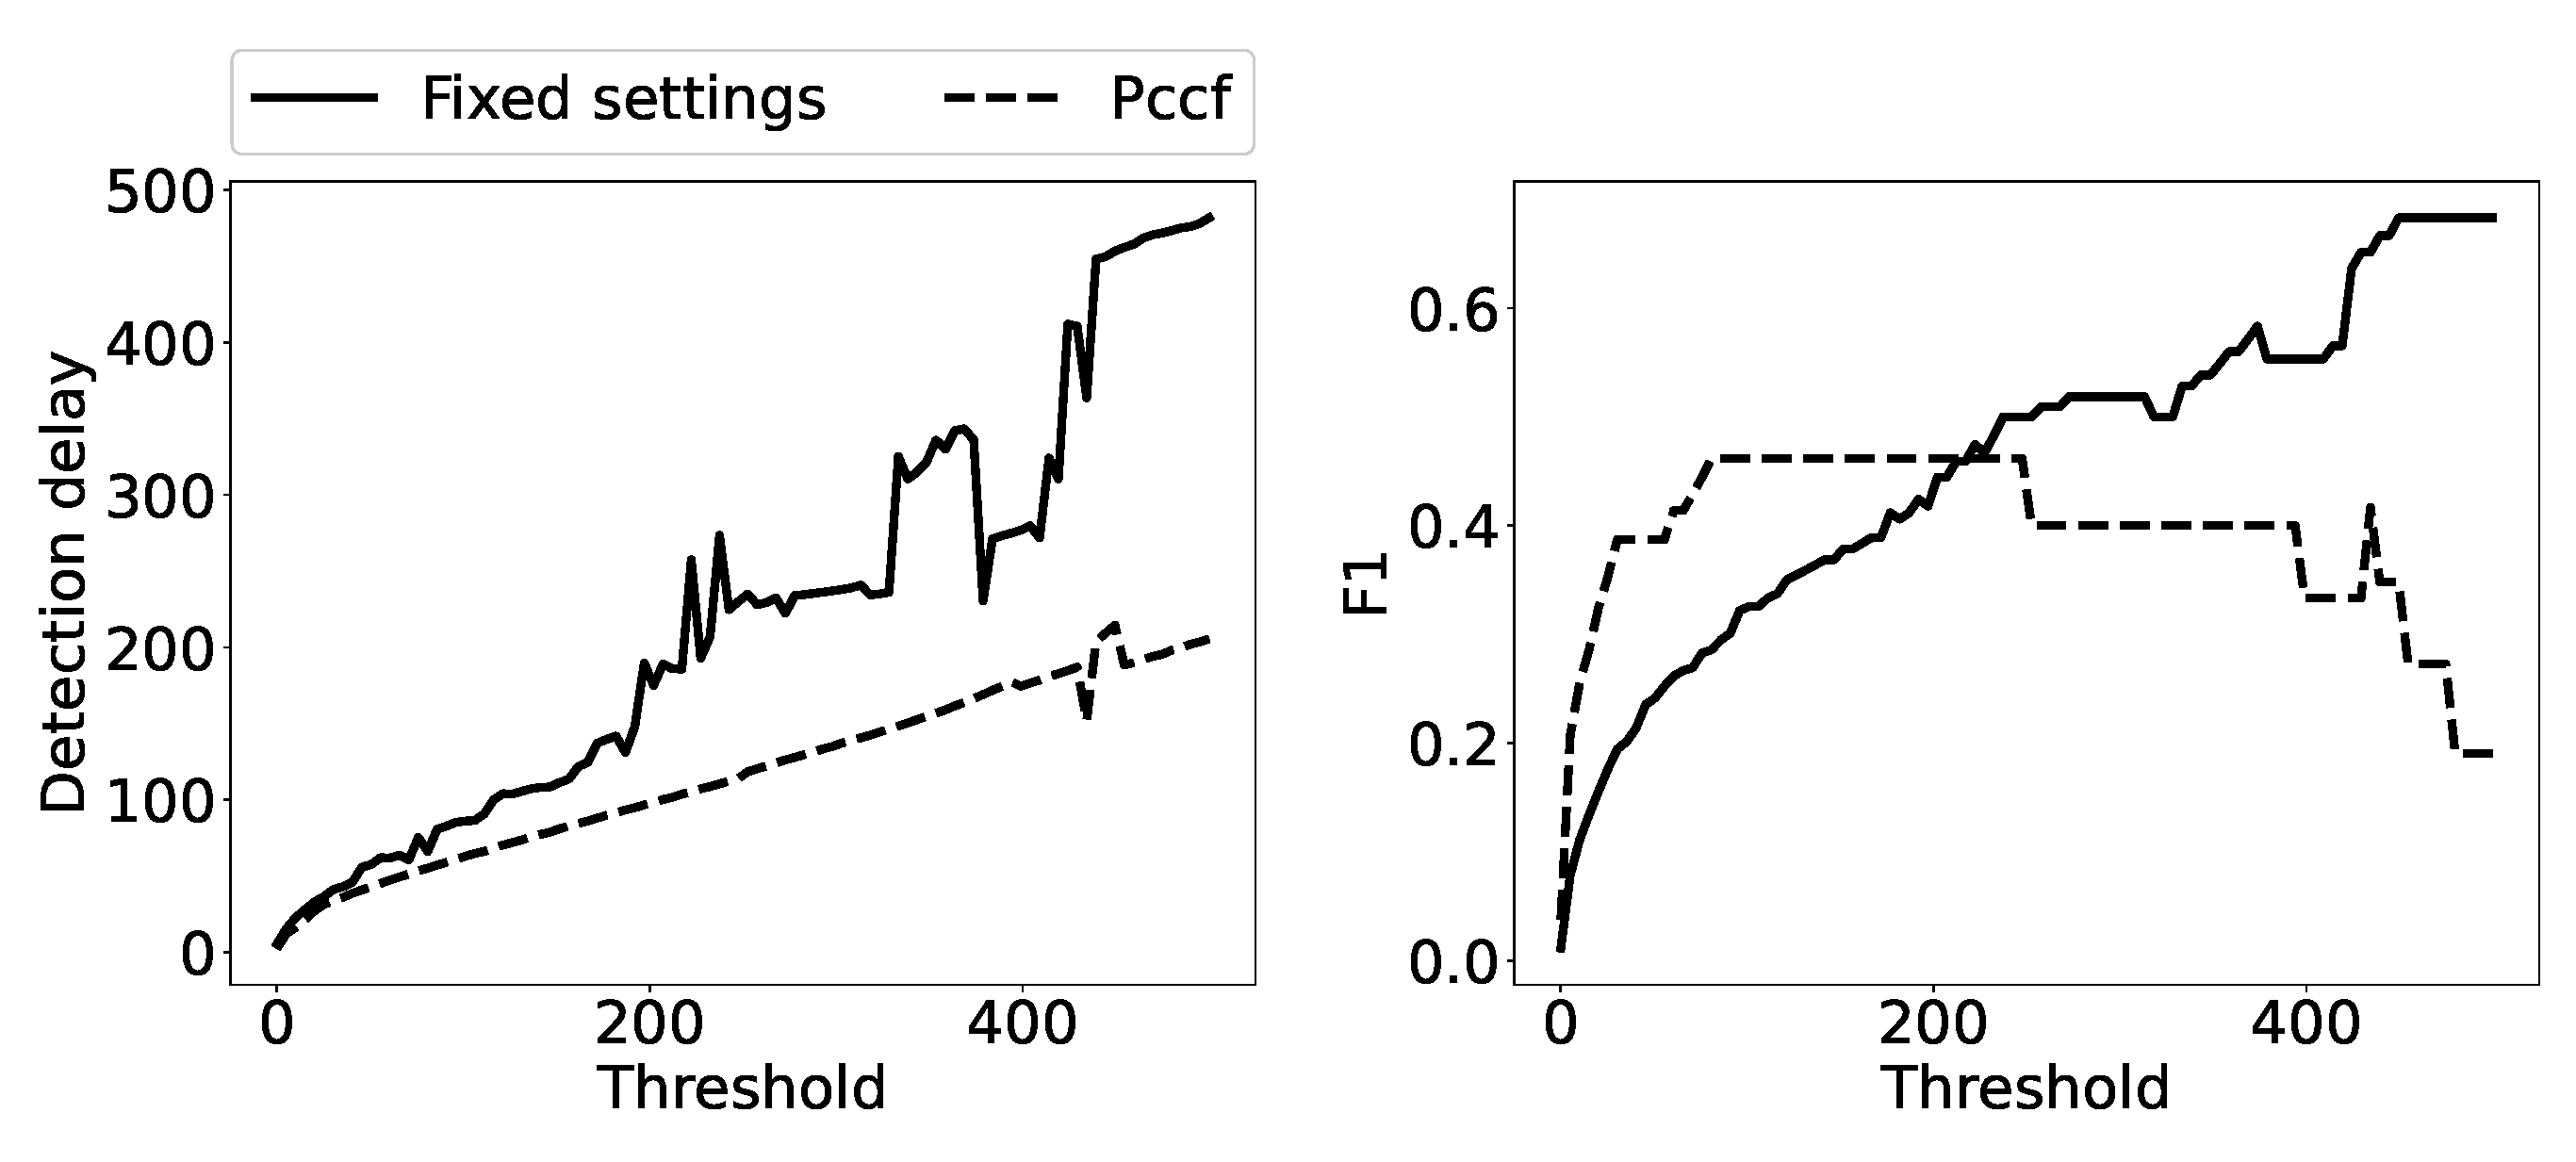
\includegraphics[width=0.8\textwidth]{articles/pics/journal_paper/performance_temperature}};
		\draw(3, 2.0) node {When predicting 7 changes};
		\draw(3, -2.7) node {When predicting all changes};
	\end{tikzpicture}
  \caption{Detection delay (left side) and $F_1$ score (right side) for the temperature signal when predicting first 7 change points (top) and when trying to predict all changes (bottom). 
  When predicting all changes $F_1$ decreases since Pccf predictions accuracy degrades with the number of change points we are trying to predict. 
  }
	\label{fig:performance_temperature_signal}
\end{figure}

